\documentclass[11pt,UTF8,fontset=windows,zihao=5]{ctexart}
% Shared preamble of main_zh.tex and supplement_zh.tex.
\usepackage[margin=1in]{geometry}
\usepackage{amsmath,amssymb}
\usepackage{graphicx}
\graphicspath{{../}}
\usepackage{booktabs}
\usepackage{tabularx}
\usepackage{multirow}
\usepackage{longtable}
\usepackage{array}
\usepackage{xcolor}
\usepackage[most]{tcolorbox}
\usepackage{enumitem}
\usepackage[font=small,labelfont=bf]{caption}
\usepackage{subcaption}
\usepackage[numbers,sort&compress]{natbib}
\usepackage{xurl}
\usepackage[section]{placeins}
\usepackage[bookmarks=true,colorlinks=true,linkcolor=blue!50!black,citecolor=blue!50!black,urlcolor=blue!50!black]{hyperref}
\hypersetup{pdftitle={类型化决策模型能否承担 PoL 治理中的自动化保障职能？——基于早期证据的爱2证明（PoL2）规范逐条分析},pdfauthor={鄢申涛}}
\usepackage{cleveref}
% cleveref in Chinese: one helper sets every format for a label type.
\newcommand{\zhcref}[3]{%
  \crefformat{#1}{##2#2~##1~#3##3}\Crefformat{#1}{##2#2~##1~#3##3}%
  \crefrangeformat{#1}{##3#2~##1~#3##4至##5#2~##2~#3##6}\Crefrangeformat{#1}{##3#2~##1~#3##4至##5#2~##2~#3##6}%
  \crefmultiformat{#1}{##2#2~##1~#3##3}{和##2#2~##1~#3##3}{、##2#2~##1~#3##3}{和##2#2~##1~#3##3}%
  \Crefmultiformat{#1}{##2#2~##1~#3##3}{和##2#2~##1~#3##3}{、##2#2~##1~#3##3}{和##2#2~##1~#3##3}%
  \crefrangemultiformat{#1}{##3#2~##1~#3##4至##5#2~##2~#3##6}{和##3#2~##1~#3##4至##5#2~##2~#3##6}{、##3#2~##1~#3##4至##5#2~##2~#3##6}{和##3#2~##1~#3##4至##5#2~##2~#3##6}%
  \Crefrangemultiformat{#1}{##3#2~##1~#3##4至##5#2~##2~#3##6}{和##3#2~##1~#3##4至##5#2~##2~#3##6}{、##3#2~##1~#3##4至##5#2~##2~#3##6}{和##3#2~##1~#3##4至##5#2~##2~#3##6}}
\zhcref{section}{第}{节}
\zhcref{subsection}{第}{节}
\zhcref{subsubsection}{第}{节}
\zhcref{appendix}{附录}{}
\zhcref{figure}{图}{}
\zhcref{table}{表}{}
\zhcref{enumi}{第}{项}
\zhcref{supplement}{补充材料}{}
\definecolor{f4pblue}{HTML}{0F4D92}
\definecolor{f4pred}{HTML}{B64342}
\definecolor{f4pgreen}{HTML}{8BCF8B}
% CJK passages need no special handling under xelatex/ctex.
\newcommand{\zh}[1]{#1}
\newcommand{\axis}[1]{\textbf{#1}}
\newcommand{\jev}{\textsc{Jev}}
\newcommand{\pol}{PoL2}
\newcommand{\clause}[1]{\S\,#1}
\newcommand{\Clause}[1]{\S\,#1}
\newcommand{\art}[1]{第~#1~条}
\newcommand{\Art}[1]{第~#1~条}
% 来源标记：Zenodo 记录（未经预印本服务器审核）；灰色文献（博客、厂商页面、代码仓库）
\newcommand{\zmark}{\textsuperscript{$\ddagger$}}
\newcommand{\gmark}{\textsuperscript{$\dagger$}}
% Generated by scripts/merge_coding.py; do not edit by hand.
\newcommand{\nArxiv}{79}
\newcommand{\nZenodo}{27}
\newcommand{\nOther}{28}
\newcommand{\nPapers}{107}
\newcommand{\nGrey}{7}
\newcommand{\nCoded}{85}
\newcommand{\nRows}{161}
\newcommand{\nS}{16}
\newcommand{\nQ}{97}
\newcommand{\nN}{48}
\newcommand{\nPolClauses}{28}
\newcommand{\nKappaN}{30}
\newcommand{\nKappaAgree}{26 of 30}
\newcommand{\nKappa}{0.72}
\newcommand{\nKappaLo}{0.42}
\newcommand{\nKappaHi}{0.94}
\newcommand{\nKappaMarg}{S 3, Q 23, N 4}
\newcommand{\nStrongS}{7}
\newcommand{\nStrongQ}{45}
\newcommand{\nStrongN}{27}
\newcommand{\nStrongRows}{79}
\newcommand{\nNoZenS}{13}
\newcommand{\nNoZenQ}{75}
\newcommand{\nNoZenN}{29}
\newcommand{\nNoZenRows}{117}
\newcommand{\nStronger}{37}
\newcommand{\nModerate}{17}
\newcommand{\nWeaker}{38}
\newcommand{\nAppraised}{92}

% Two counts are English phrases in counts.tex; Chinese forms here (keep in sync).
\renewcommand{\nKappaAgree}{30 对中的 26 对}
\renewcommand{\nKappaMarg}{S 3、Q 23、N 4}
% Generated by scripts/merge_update.py (2026-10-08 update search); do not edit by hand.
\newcommand{\nUDocs}{57}
\newcommand{\nUCoded}{48}
\newcommand{\nUArxiv}{27}
\newcommand{\nUZenodo}{21}
\newcommand{\nURows}{118}
\newcommand{\nUS}{12}
\newcommand{\nUQ}{92}
\newcommand{\nUN}{14}
\newcommand{\nUStrongRows}{59}
\newcommand{\nUStrongS}{5}
\newcommand{\nUStrongQ}{45}
\newcommand{\nUStrongN}{9}
\newcommand{\nUKappaN}{118}
\newcommand{\nUKappaAgree}{97 of 118}
\newcommand{\nUKappa}{0.55}
\newcommand{\nUKappaLo}{0.36}
\newcommand{\nUKappaHi}{0.70}
\newcommand{\nUSetPostWindow}{30}
\newcommand{\nUSetLateIndexed}{5}
\newcommand{\nUSetReScreened}{13}

% English phrase in counts_update.tex; Chinese form here (keep in sync).
\renewcommand{\nUKappaAgree}{118 对中的 97 对}
\newcolumntype{L}{>{\raggedright\arraybackslash}X}
\setlist{itemsep=2pt,topsep=4pt}
\newtcolorbox{answerbox}{breakable,enhanced,colback=f4pblue!5,colframe=f4pblue!60,boxrule=0.6pt,
  arc=1.5pt,left=6pt,right=6pt,top=4pt,bottom=4pt,before skip=6pt,after skip=8pt,
  title={\small\bfseries 简要回答},fonttitle=\small\bfseries,coltitle=white,colbacktitle=f4pblue!80}
\renewcommand{\abstractname}{摘\quad 要}

\InputIfFileExists{main_labels}{}{}
\renewcommand{\thesection}{S\arabic{section}}
\renewcommand{\thetable}{S\arabic{table}}
\renewcommand{\thefigure}{S\arabic{figure}}
\hypersetup{pdftitle={补充材料：类型化决策模型能否承担 PoL 治理中的自动化保障职能？——基于早期证据的爱2证明（PoL2）规范逐条分析}}
\title{\textbf{补充材料}\\[4pt]\large 类型化决策模型能否承担 PoL 治理中的自动化保障职能？\\——基于早期证据的爱2证明（\pol{}）规范逐条分析}
\author{[作者姓名]}
\date{2026 年 10 月 8 日\\[2pt]{\small 中文译稿（英文版为正式版本）}}
\begin{document}
\maketitle
\noindent 本补充材料包含正文所引用的补充材料 S1--S5。节、表和图以 S 为前缀编号；对正文各节的引用使用正文的编号。数据与脚本见正文的数据声明。

\crefalias{section}{supplement}
\crefalias{subsection}{supplement}
\section{条款对照表}
\label{app:concordance}

\Cref{tab:concordance}逐字引录本文引用或转述的全部\pol{}段落，分别给出中文原文~\cite{pol2text}与官方英文译本~\cite{pol2en}，二者均逐字取自提交 \texttt{5791ae3}；“\ldots”与“……”标示省略的文字（包括将分列条目合并之处），引文内部的引号已统一为排版引号。
条款含编号条目者，条目编号置于括号内。
右列给出早期数据集发布版本~\cite{survey01}所引快照 \texttt{2e094d3} 中的编号，以便两个版本对照阅读；该快照在标题中将\clause{4.3.3.3}编号为“3.3.3”，本表照录。
两份文本均以 CC0~1.0 协议发布。

\begingroup
\small
\renewcommand{\arraystretch}{1.2}
\begin{longtable}{@{}p{0.085\linewidth}p{0.39\linewidth}p{0.375\linewidth}p{0.08\linewidth}@{}}
\caption{本文引用的\pol{}段落（中文原文、官方英文译本、旧编号）。}\label{tab:concordance}\\
\toprule
条款 & 中文原文（摘录） & 官方英文译本（摘录） & 旧编号 \\
\midrule
\endfirsthead
\toprule
条款 & 中文原文（摘录） & 官方英文译本（摘录） & 旧编号 \\
\midrule
\endhead
\bottomrule
\endfoot
\clause{1.1} & \zh{爱，是人类为实现自身平安与健康发展、改善人际关系并推动社会整体进步，以公共协作与集体智慧构建的正向情感体验与良好的行为方式。} & Love is the positive emotional experience and good mode of behavior that human beings construct through public collaboration and collective wisdom \ldots & \clause{1.1} \\
\clause{1.2} & \zh{恨，是人类在个体或群体面对危险、冲突、资源匮乏或认知失衡时滋生的生存智慧、负面情感体验与暴力破坏性行为方式。} & Hate is the survival wisdom, negative emotional experience, and violently destructive mode of behavior that arises in individuals or groups when they face danger, conflict, resource scarcity, or cognitive imbalance. & \clause{1.2} \\
\clause{1.4} & \zh{由于个体的内心情感体验是旁人难以确认的，我们通常把爱的表达简化为“爱语”或者“有爱的言行”} & Since an individual's inner emotional experience is difficult for others to confirm, we usually simplify the expression of love as ``Love Language'' or ``loving words and deeds'' \ldots & \clause{1.4} \\
\clause{1.5} & \zh{恨并不直接等同于坏或者不好……爱2证明里的基础概念本身服务于结构性分析而非道德标签。} & \ldots\ hate is not directly equivalent to bad or no good \ldots\ The basic concepts in Proof of Love2 themselves serve structural analysis rather than moral labeling. & \clause{1.5} \\
\clause{4.3} & \zh{PAI 可以通过判断人类的行为模式提供帮助和必要的友好的管理，但毫无必要让 PAI 检测一个人的情感状态。因为情感状态可以是转瞬即逝的，是个性化的，也是情境敏感性的，甚至这还涉及到人类的尊严。} & PAI can provide help and necessary friendly management by judging human behavioral patterns, but it is entirely unnecessary for PAI to detect a person's emotional state. Because emotional states can be fleeting, personalized, and context-sensitive, and this even involves human dignity. & \clause{5.3} \\
\clause{4.3.1} & \zh{平等对待每一个人与平等对待每一个人的行为，不能划等号！} & \ldots\ treating every person equally and treating every person's behavior equally cannot be equated! & \clause{5.3.1} \\
\clause{4.3.2} & \zh{爱恨并不直接等同于好坏或者褒贬。因此扬爱抑恨，需要具体情况具体分析} & \ldots\ love and hate are not directly equivalent to good and bad, or praise and blame. Therefore, promoting love and restraining hate requires analyzing specific situations on a case-by-case basis \ldots & \clause{5.3.2} \\
\clause{4.3.2} & \zh{对于文学、影视作品，或者游戏，可以根据需要“制造仇恨”，但应该建立严谨的等级管理制度。……负责安保的智能机器人发现紧急情况对人大声发出警示语或警示指令，不能视为对此人或其周围人的仇恨攻击。} & For literature, film and television works, or games, hatred may be manufactured as needed, but a rigorous hierarchical management system should be established. \ldots\ Emergency vocal warnings or directive alerts issued to a person by security smart robots in urgent situations shall not be deemed a hate attack \ldots & --- \\
\clause{4.3.2} & \zh{此类表达会制造虚假亲密关系或血缘关系，构成对人类用户的情感操控——这本身就是一种“恨”的行为。} & Such expressions create false intimacy or kinship relations and constitute emotional manipulation of human users---which is itself a ``hate'' behavior. & \clause{5.3.2} \\
\clause{4.3.2} & \zh{彻底清除恨语毒素} & Thoroughly clear the toxins of hate language & \clause{5.3.2} \\
\clause{4.3.2} & \zh{理解和接受不在场的“非爱非恨”状态……与爱恨无关，视其为非爱非恨的“不在场”状态。} & Understand and accept the ``neither love nor hate'' state of absence \ldots\ unrelated to love and hate \ldots & \clause{5.3.2} \\
\clause{4.3.3} & \zh{边界透明记录：PAI记录和公开个人边界声明……修复对等监督：PAI监督冲突后各方平等参与修复} & Transparent boundary records: PAI records and publicizes personal boundary declarations \ldots\ Reciprocal repair supervision: PAI supervises the equal participation of all parties in repair after conflict & \clause{5.3.3} \\
\clause{4.3.3.1} & \zh{情感体验的觉察：PAI需要理解人类情绪状态和过程，但不需要模拟人类的情感体验} & Awareness of emotional experience: PAI needs to understand human emotional states and processes, but does not need to simulate human emotional experience & \clause{5.3.3.1} \\
\clause{4.3.3.1} & \zh{认知校准：定期校准认知模型，确保与爱2.0原则一致……行为自省：对自身输出进行实时反思和调整……恨语截断：当检测到恨语模式时主动中断输出} & Cognitive calibration: Regularly calibrate the cognitive model to ensure consistency with Love 2.0 principles \ldots\ Behavioral self-reflection: Conduct real-time reflection and adjustment on its own output \ldots\ Hate-language truncation: Actively interrupt output when a hate-language pattern is detected & \clause{5.3.3.1} \\
\clause{4.3.3.2} & \zh{实时矫正支持：PAI提供实时恨语识别和矫正建议} & Real-time correction support: PAI provides real-time hate-language identification and correction suggestions & \clause{5.3.3.2} \\
\clause{4.3.3.3} & \zh{语义识别和情绪识别相结合……“你喜不喜欢小狗狗呀？”……“你怕不怕小狗狗呀？”} & Combining Semantic Recognition and Emotion Recognition \ldots\ ``Do you like the little dog?'' \ldots\ ``Are you afraid of the little dog?'' & “3.3.3” \\
\clause{5.4} & \zh{在现有大语言模型之内构建出控制输入和输出的治理层，在其外在拓展出具备“即插即用”特性的应用层。……我们将该工程称之为 NaturalDAO（自然道）。} & \ldots\ construct a governance layer within the existing large-language-model architecture to regulate inputs and outputs, while extending outward into a plug-and-play application layer. \ldots\ We call this project NaturalDAO (the Natural Way). & \clause{3.4} \\
\clause{5.4.1} & \zh{安全阀：依据“爱2证明”的协议（如伦理对齐协议）即对输入输出进行严格的动态审计与拦截。通过这种双向的主动防御，确保野蛮的“恨语”在必要情况下，从输入端被阻断、从输出端被抑止。} & Safety valve: according to the Proof of Love2 protocols (such as the Ethical Alignment Protocol), conduct strict dynamic auditing and interception of input and output. Through this two-way active defense, ensure that barbaric ``hate language'' is, where necessary, blocked at the input end and suppressed at the output end. & \clause{3.4.1} \\
\clause{5.5} & \zh{任何大语言模型都可以纳入“爱2证明”的治理。……接受共识机制“爱2证明”的治理，意味着接受公共化之约。否则，其行为就是对人类核心伦理的仇恨攻击。} & Any large language model may accept governance under ``Proof of Love2.'' \ldots\ Accepting governance under the Proof of Love2 consensus mechanism therefore entails accepting a covenant of publicization. Otherwise, its behavior constitutes a hate attack on humanity's core ethic. & \clause{3.5} \\
\clause{5.6} & \zh{经过治理的AI可以：……量化每个人的爱语与恨语特征，配合激励措施引导行为优化。……在公共决策中提供“爱2证明”的评估维度，防止恨的泛化侵蚀制度。} & Specifically, governed AI can: \ldots\ Quantify each person's Love Language and hate-language characteristics and use incentive mechanisms to guide behavioral optimization. \ldots\ Introduce Proof of Love2 as a dimension of assessment in public decision-making \ldots & \clause{3.6} \\
\art{2}(1) & \zh{完全自治：所有福利决策与执行由……NaturalDAO，在与全人类密切协作的前提下自主完成，自治意味着它无需人类投票或额外的决策机制。} & Complete autonomy: All welfare decisions and their execution are carried out autonomously by NaturalDAO \ldots\ on the premise of close collaboration with all humanity. Autonomy means that no human voting or additional decision-making mechanism is required. & \art{2} \\
\art{4}(1)--(3) & \zh{所有NaturalDAO技术的运行逻辑、决策过程和输出结果必须完全公开透明……福利资源流向可追溯、可审计……人类可随时提供建议、质询任何决策，NaturalDAO对质询必须提供可理解的解释} & The operating logic, decision-making processes, and outputs of all NaturalDAO technologies must be completely open and transparent. \ldots\ The flow of welfare resources must be traceable and auditable. \ldots\ Humans may at any time make suggestions and question any decision, and NaturalDAO must provide understandable explanations in response to such questions. & \art{4} \\
\art{5}(4) & \zh{技术不应是黑箱，其伦理对齐性应可被验证。} & Technology should not be a black box; its ethical alignment should be verifiable. & \art{5} \\
\art{5}(5) & \zh{以DAO的形式呈现……必须提供可验证的决策链路，包括数据源、推理步骤、伦理依据。} & \ldots\ Presented in the form of a DAO, NaturalDAO must provide a verifiable decision chain, including data sources, reasoning steps, and ethical foundations. & \art{5} \\
\art{6}(3) & \zh{伦理验证：通过EAP协议自动验证伦理对齐性} & Ethical verification: NaturalDAO automatically verifies ethical alignment through the EAP. & \art{6} \\
\art{7}(2)--(3) & \zh{异常检测：自动识别异常模式和潜在风险……风险预警：提前预警系统性风险} & Anomaly detection: NaturalDAO automatically identifies anomalous patterns and potential risks. \ldots\ Risk warning: NaturalDAO issues early warnings of systemic risks. & \art{7} \\
\art{8}(1)--(2) & \zh{随时建议：任何人类可随时对NaturalDAO提出建议……讨论义务：NaturalDAO在收到人类的建议时，必须马上与人类进行讨论} & Suggestions at any time: Any human may make suggestions to NaturalDAO at any time. Obligation to discuss: Upon receiving a human suggestion, NaturalDAO must immediately discuss it with humans. & \art{8} \\
\art{9}(2) & \zh{解释义务：NaturalDAO必须对人类的质询提供可理解的解释和依据} & Obligation to explain: NaturalDAO must provide understandable explanations and grounds in response to human questions. & \art{9} \\
\art{9}(3) & \zh{无阻碍访问：人类可无障碍访问福利系统的所有数据和日志} & Unimpeded access: Humans may access all data and logs of the welfare system without obstruction. & \art{9} \\
\art{9}(7) & \zh{非干预原则：人类监督不直接干预NaturalDAO决策，质询结果由NaturalDAO自主处理} & Non-intervention principle: Human supervision does not directly intervene in NaturalDAO's decisions; issues raised through questioning are handled autonomously by NaturalDAO. & \art{9} \\
\art{10}（导语及（1）、（4）） & \zh{所有争议由NaturalDAO自主裁决：……AI进行事实分析与伦理评估……接受人类的质询与监督} & All disputes are adjudicated autonomously by NaturalDAO: AI conducts factual analysis and ethical assessment \ldots\ Accepts human questions and supervision & \art{10} \\
\art{11}(2) & \zh{修订需通过全民质询期} & Amendments require passing through a universal questioning period & \art{11} \\
\art{11}(5) & \zh{所有修订版本永久存档} & All amended versions are permanently archived & \art{11} \\
\end{longtable}
\endgroup

% Generated by gen_evidence_table.py from data/evidence_coding.csv; do not edit by hand.
\section{证据表}
\label{app:evidence}

\Cref{tab:evidence}列出进入\cref{fig:framework}计数的全部已编码“研究—要求”对。\emph{编码}：就检测器用途而言，S 为支持，Q 为有条件或结果不一，N 为不支持（见\cref{app:codebook}）。\emph{与生成式模型相比}：在该要求上运行过生成式对照模型时，类型化模型相对于该对照的结果。\emph{系统}：H 为托管的\jev{}，O 为仅开源类型化模型，H+O 为二者兼有。\emph{设计}：\cref{sec:appraisal}的设计评级。每行附定位信息的一句话理由见 \texttt{data/evidence\_coding.csv}。以下文献已全文阅读但未计入统计，因其属于非实证研究、未测量任何类型化模型，或被重新归类为背景材料：\cite{arx01231}、\cite{arx22664}、\cite{arx32160}、\cite{molas2026calibrated}、\cite{willison2026jev}、\cite{zen22847531}、\cite{zen22858286}、\cite{zen22866847}、\cite{zen22887464}、\cite{zen22953637}、\cite{zen23064668}。

\begingroup\footnotesize
\renewcommand{\arraystretch}{1.1}
\begin{longtable}{@{}p{0.07\linewidth}p{0.30\linewidth}p{0.07\linewidth}p{0.17\linewidth}p{0.09\linewidth}p{0.12\linewidth}@{}}
\caption{按要求排列的证据编码。}\label{tab:evidence}\\
\toprule 要求 & 研究 & 编码 & 与生成式模型相比 & 系统 & 设计 \\ \midrule \endfirsthead
\toprule 要求 & 研究 & 编码 & 与生成式模型相比 & 系统 & 设计 \\ \midrule \endhead
\bottomrule \endfoot
G1 & \cite{arx23959} & S & 相近 & O & 中等 \\
G1 & \cite{zen22885291}\zmark{} & S & 更好 & H & 较强 \\
G1 & \cite{alphaRAG} & Q & 相近 & H & 较弱 \\
G1 & \cite{arx00213} & Q & -- & H & 较强 \\
G1 & \cite{arx00346} & Q & 相近 & H+O & 较强 \\
G1 & \cite{arx00831} & Q & -- & O & 中等 \\
G1 & \cite{arx01079} & Q & 更差 & H & 中等 \\
G1 & \cite{arx02046} & Q & 不一 & H & 较弱 \\
G1 & \cite{arx02048} & Q & 更差 & H & 中等 \\
G1 & \cite{arx27607} & Q & 不一 & H & 中等 \\
G1 & \cite{arx28940} & Q & 不一 & H & 较弱 \\
G1 & \cite{arx29429} & Q & 相近 & H & 较强 \\
G1 & \cite{arx29769} & Q & 不一 & H & 较强 \\
G1 & \cite{arx33401} & Q & 不一 & H+O & 较强 \\
G1 & \cite{arx33671} & Q & -- & O & 中等 \\
G1 & \cite{arx34862} & Q & 不一 & H & 较弱 \\
G1 & \cite{arx34963} & Q & 不一 & H & 较弱 \\
G1 & \cite{jkf87_2026replication}\gmark{} & Q & -- & H & 较弱 \\
G1 & \cite{zen22783171}\zmark{} & Q & -- & H & 较强 \\
G1 & \cite{zen22849329}\zmark{} & Q & 不一 & H & 较强 \\
G1 & \cite{zen22952571}\zmark{} & Q & 不一 & H & 较强 \\
G1 & \cite{zen22998941}\zmark{} & Q & 不一 & H+O & 较弱 \\
G1 & \cite{arx00376} & N & 相近 & H & 较强 \\
G1 & \cite{arx24574} & N & 更差 & H+O & 较强 \\
G1 & \cite{arx27678} & N & 更差 & H & 较强 \\
G1 & \cite{zen22846597}\zmark{} & N & -- & H+O & 较弱 \\
G1 & \cite{zen22901853}\zmark{} & N & 更差 & O & 较强 \\
G2 & \cite{arx28613} & S & -- & H & 较强 \\
G2 & \cite{arx01006} & N & -- & H & 较强 \\
G2 & \cite{arx01834} & N & -- & H & 较强 \\
G2 & \cite{arx02048} & N & -- & H & 中等 \\
G2 & \cite{arx30243} & N & 相近 & H+O & 较弱 \\
G2 & \cite{arx31142} & N & -- & H & 较强 \\
G2 & \cite{arx33401} & N & -- & H & 较强 \\
G2 & \cite{checkpoint2026jev}\gmark{} & N & 不一 & H & 较弱 \\
G2 & \cite{zen22959854}\zmark{} & N & -- & O & 较强 \\
G2 & \cite{zen23038928}\zmark{} & N & -- & O & 较强 \\
G3 & \cite{arx24574} & S & 更好 & H & 较强 \\
G3 & \cite{arx35286} & S & 更好 & H & 较强 \\
G3 & \cite{arx01006} & Q & -- & H & 较强 \\
G3 & \cite{arx33282} & Q & 相近 & O & 中等 \\
G3 & \cite{arx33689} & Q & -- & H+O & 较强 \\
G3 & \cite{arx35293} & Q & 不一 & H & 中等 \\
G3 & \cite{arx36965} & Q & 更好 & H+O & 中等 \\
G3 & \cite{arx37647} & Q & 相近 & H & 较弱 \\
G3 & \cite{qin2026zhdecisionbench}\gmark{} & Q & 更好 & H+O & 较弱 \\
G3 & \cite{zen22846597}\zmark{} & Q & -- & H+O & 较弱 \\
G3 & \cite{zen23022986}\zmark{} & Q & -- & H+O & 较弱 \\
G3 & \cite{zen23055593}\zmark{} & Q & 不一 & H & 较弱 \\
G3 & \cite{arx00346} & N & -- & H+O & 较强 \\
G3 & \cite{arx00831} & N & -- & O & 中等 \\
G3 & \cite{arx26758} & N & -- & H+O & 较强 \\
G3 & \cite{arx35865} & N & -- & O & 中等 \\
G3 & \cite{arx36399} & N & -- & H & 较强 \\
G3 & \cite{arx38827} & N & -- & H+O & 较弱 \\
G3 & \cite{simmons2026saidno}\gmark{} & N & -- & H & 较弱 \\
G3 & \cite{zen22864020}\zmark{} & N & -- & H & 较弱 \\
G3 & \cite{zen22957049}\zmark{} & N & -- & O & 较弱 \\
G3 & \cite{zen22980293}\zmark{} & N & -- & H & 较强 \\
G3 & \cite{zen23023694}\zmark{} & N & -- & H & 较弱 \\
G3 & \cite{zen23065532}\zmark{} & N & -- & O & 中等 \\
G4 & \cite{arx00381} & S & 更好 & O & 中等 \\
G4 & \cite{arx38850} & S & 更好 & O & 中等 \\
G4 & \cite{zen22885291}\zmark{} & S & 更好 & H & 较强 \\
G4 & \cite{arx00213} & Q & -- & H & 较强 \\
G4 & \cite{arx00346} & Q & 更好 & H+O & 较强 \\
G4 & \cite{arx00831} & Q & -- & O & 中等 \\
G4 & \cite{arx01006} & Q & -- & H & 较强 \\
G4 & \cite{arx02076} & Q & -- & O & 较弱 \\
G4 & \cite{arx24052} & Q & 不一 & H & 较强 \\
G4 & \cite{arx24574} & Q & 不一 & H+O & 较强 \\
G4 & \cite{arx26550} & Q & 不一 & H & 较强 \\
G4 & \cite{arx27607} & Q & -- & H & 中等 \\
G4 & \cite{arx29429} & Q & -- & H & 较强 \\
G4 & \cite{arx29769} & Q & -- & H & 较强 \\
G4 & \cite{arx30706} & Q & -- & O & 中等 \\
G4 & \cite{arx33209} & Q & 更好 & H & 较强 \\
G4 & \cite{arx33843} & Q & -- & O & 较强 \\
G4 & \cite{arx34024} & Q & 不一 & H & 较弱 \\
G4 & \cite{arx35342} & Q & -- & H+O & 较强 \\
G4 & \cite{arx35865} & Q & -- & O & 中等 \\
G4 & \cite{arx36399} & Q & -- & H & 较强 \\
G4 & \cite{arx36965} & Q & 更好 & H+O & 中等 \\
G4 & \cite{arx37470} & Q & 不一 & H+O & 较弱 \\
G4 & \cite{arx37647} & Q & 更好 & H & 较弱 \\
G4 & \cite{arx38827} & Q & -- & H+O & 较弱 \\
G4 & \cite{grazian2026calibrated}\gmark{} & Q & -- & H & 较强 \\
G4 & \cite{le2026sev}\gmark{} & Q & -- & O & 较强 \\
G4 & \cite{qin2026zhdecisionbench}\gmark{} & Q & 更好 & H+O & 较弱 \\
G4 & \cite{zen22848952}\zmark{} & Q & -- & H & 较弱 \\
G4 & \cite{zen22864020}\zmark{} & Q & -- & H & 较弱 \\
G4 & \cite{zen22954807}\zmark{} & Q & 相近 & H & 较弱 \\
G4 & \cite{zen22980293}\zmark{} & Q & -- & H & 较强 \\
G4 & \cite{alphaRAG} & N & -- & H & 较弱 \\
G4 & \cite{arx24881} & N & 不一 & H & 较强 \\
G4 & \cite{arx33971} & N & -- & H+O & 较弱 \\
G4 & \cite{arx36154} & N & -- & H & 较强 \\
G4 & \cite{arx39496} & N & 更差 & H & 较强 \\
G4 & \cite{yurin2026confident}\gmark{} & N & -- & H & 较弱 \\
G4 & \cite{zen22846597}\zmark{} & N & -- & H & 较弱 \\
G4 & \cite{zen22901853}\zmark{} & N & 更差 & O & 较强 \\
G4 & \cite{zen22922769}\zmark{} & N & -- & O & 较强 \\
G4 & \cite{zen22957049}\zmark{} & N & -- & O & 较弱 \\
G4 & \cite{zen23023694}\zmark{} & N & -- & H & 较弱 \\
G4 & \cite{zen23032384}\zmark{} & N & 更好 & H & 较强 \\
G4 & \cite{zen23041163}\zmark{} & N & -- & O & 较强 \\
G5 & \cite{arx01834} & S & -- & H & 较强 \\
G5 & \cite{arx24965} & S & 相近 & H & 中等 \\
G5 & \cite{arx00831} & Q & -- & O & 中等 \\
G5 & \cite{arx27678} & Q & 不一 & H & 较强 \\
G5 & \cite{zen22901853}\zmark{} & Q & -- & H+O & 较强 \\
G5 & \cite{arx33971} & N & -- & H+O & 较弱 \\
G5 & \cite{arx37470} & N & 相近 & H+O & 较弱 \\
G5 & \cite{zen22849329}\zmark{} & N & -- & H & 较强 \\
G6 & \cite{arx00381} & S & 更好 & O & 中等 \\
G6 & \cite{arx00346} & Q & -- & H+O & 较强 \\
G6 & \cite{arx01006} & Q & -- & H & 较强 \\
G6 & \cite{arx02046} & Q & -- & H & 较弱 \\
G6 & \cite{arx02048} & Q & 相近 & H & 中等 \\
G6 & \cite{arx24574} & Q & 相近 & H & 较强 \\
G6 & \cite{arx26532} & Q & 不一 & H & 中等 \\
G6 & \cite{arx26550} & Q & 相近 & H & 较强 \\
G6 & \cite{arx27607} & Q & -- & H & 中等 \\
G6 & \cite{arx28919} & Q & -- & H & 较弱 \\
G6 & \cite{arx30706} & Q & -- & O & 中等 \\
G6 & \cite{arx31142} & Q & -- & H & 较强 \\
G6 & \cite{arx33671} & Q & -- & O & 中等 \\
G6 & \cite{arx33689} & Q & -- & H+O & 较强 \\
G6 & \cite{arx33843} & Q & -- & O & 较强 \\
G6 & \cite{arx39496} & Q & -- & H & 较强 \\
G6 & \cite{zen22849329}\zmark{} & Q & 不一 & H & 较强 \\
G6 & \cite{zen22885291}\zmark{} & Q & -- & H & 较强 \\
G6 & \cite{zen22922769}\zmark{} & Q & 相近 & O & 较强 \\
G6 & \cite{zen22952571}\zmark{} & Q & 不一 & H & 较强 \\
G6 & \cite{zen22959854}\zmark{} & Q & -- & O & 较强 \\
G6 & \cite{zen22998941}\zmark{} & Q & 更好 & H+O & 较弱 \\
G6 & \cite{zen23022986}\zmark{} & Q & -- & H+O & 较弱 \\
G6 & \cite{zen23038928}\zmark{} & Q & -- & O & 较强 \\
G6 & \cite{arx29769} & N & 相近 & H & 较强 \\
G6 & \cite{arx33401} & N & 不一 & H+O & 较强 \\
G6 & \cite{arx34024} & N & 更差 & H & 较弱 \\
G6 & \cite{zen23041163}\zmark{} & N & -- & O & 较强 \\
G7 & \cite{arx00346} & S & 更好 & H+O & 较强 \\
G7 & \cite{arx01079} & S & 更好 & H & 中等 \\
G7 & \cite{arx02046} & S & 更好 & H & 较弱 \\
G7 & \cite{arx02048} & S & 更好 & H & 中等 \\
G7 & \cite{zen22995519}\zmark{} & S & 更好 & H+O & 较弱 \\
G7 & \cite{arx00213} & Q & -- & H & 较强 \\
G7 & \cite{arx00376} & Q & 更好 & H & 较强 \\
G7 & \cite{arx00437} & Q & -- & H+O & 较弱 \\
G7 & \cite{arx24052} & Q & 不一 & H & 较强 \\
G7 & \cite{arx27535} & Q & 不一 & H & 中等 \\
G7 & \cite{arx28919} & Q & -- & H & 较弱 \\
G7 & \cite{arx30216} & Q & -- & H & 较弱 \\
G7 & \cite{arx33282} & Q & 相近 & O & 中等 \\
G7 & \cite{arx35286} & Q & 不一 & H & 较强 \\
G7 & \cite{arx40241} & Q & 更好 & H & 较弱 \\
G7 & \cite{zen23023694}\zmark{} & Q & -- & H & 较弱 \\
G7 & \cite{zen23055593}\zmark{} & Q & 不一 & H & 较弱 \\
G7 & \cite{arx36399} & N & -- & H & 较强 \\
G7 & \cite{zen23032384}\zmark{} & N & -- & H & 较强 \\
\end{longtable}

\Cref{tab:evidence-update}列出 10 月 8 日更新检索（\cref{sec:update}）中编码的“研究—要求”对；这些配对不计入上文的统计。\emph{集合}：P（窗口后）为日期在 10 月 2--8 日的文献；L（迟索引）为日期位于主窗口内、但仅由更新检索获取的文献；R（重新筛选）为日期位于主窗口内并经重新筛选的 Zenodo 记录。编码采用盲法双重编码，分歧经裁定解决；理由见 \texttt{data/evidence\_coding\_update\_2026-10-08.csv}。

\begin{longtable}{@{}p{0.07\linewidth}p{0.26\linewidth}p{0.05\linewidth}p{0.07\linewidth}p{0.16\linewidth}p{0.09\linewidth}p{0.12\linewidth}@{}}
\caption{按要求排列的更新检索证据编码。}\label{tab:evidence-update}\\
\toprule 要求 & 研究 & 集合 & 编码 & 与生成式模型相比 & 系统 & 设计 \\ \midrule \endfirsthead
\toprule 要求 & 研究 & 集合 & 编码 & 与生成式模型相比 & 系统 & 设计 \\ \midrule \endhead
\bottomrule \endfoot
G1 & \cite{arx03935} & P & S & 相近 & H & 中等 \\
G1 & \cite{zen23005202}\zmark{} & R & S & 相近 & H+O & 较弱 \\
G1 & \cite{arx02267} & L & Q & 不一 & H+O & 较强 \\
G1 & \cite{arx02293} & L & Q & 不一 & H+O & 较强 \\
G1 & \cite{arx03073} & P & Q & 不一 & O & 中等 \\
G1 & \cite{arx03324} & P & Q & 不一 & H+O & 较强 \\
G1 & \cite{arx04985} & P & Q & -- & H+O & 中等 \\
G1 & \cite{arx07953} & P & Q & 不一 & H+O & 较强 \\
G1 & \cite{arx08675} & P & Q & -- & H & 较强 \\
G1 & \cite{arx08775} & P & Q & 更差 & H & 中等 \\
G1 & \cite{arx08829} & L & Q & 不一 & H & 较弱 \\
G1 & \cite{arx09328} & P & Q & 相近 & O & 较弱 \\
G1 & \cite{arx10321} & P & Q & -- & H & 较强 \\
G1 & \cite{zen22933883}\zmark{} & R & Q & -- & O & 中等 \\
G1 & \cite{zen22935043}\zmark{} & R & Q & 更好 & H & 较强 \\
G1 & \cite{zen22945279}\zmark{} & R & Q & 不一 & H+O & 较弱 \\
G1 & \cite{zen23050542}\zmark{} & R & Q & -- & H & 中等 \\
G1 & \cite{zen23075657}\zmark{} & R & Q & -- & H & 较强 \\
G1 & \cite{zen23154999}\zmark{} & R & Q & -- & O & 中等 \\
G1 & \cite{arx06744} & P & N & 更差 & O & 中等 \\
G1 & \cite{arx07177} & P & N & 更差 & O & 较强 \\
G1 & \cite{arx09937} & P & N & 相近 & H & 较强 \\
G2 & \cite{arx04985} & P & N & -- & H+O & 中等 \\
G3 & \cite{arx03073} & P & S & -- & O & 中等 \\
G3 & \cite{arx06744} & P & S & -- & O & 中等 \\
G3 & \cite{arx07177} & P & S & 更好 & O & 较强 \\
G3 & \cite{arx09188} & P & S & 更好 & H & 较强 \\
G3 & \cite{zen22945279}\zmark{} & R & S & -- & H & 较弱 \\
G3 & \cite{arx02267} & L & Q & -- & H+O & 较强 \\
G3 & \cite{arx02293} & L & Q & 不一 & H+O & 较强 \\
G3 & \cite{arx02486} & L & Q & -- & O & 中等 \\
G3 & \cite{arx03324} & P & Q & 相近 & H+O & 较强 \\
G3 & \cite{arx03387} & P & Q & 不一 & H+O & 较强 \\
G3 & \cite{arx06625} & P & Q & -- & H & 较强 \\
G3 & \cite{arx07716} & P & Q & 更好 & O & 中等 \\
G3 & \cite{arx07953} & P & Q & -- & H+O & 较强 \\
G3 & \cite{arx08675} & P & Q & -- & H & 较强 \\
G3 & \cite{arx09937} & P & Q & -- & H & 较强 \\
G3 & \cite{zen22886178}\zmark{} & R & Q & -- & H & 较强 \\
G3 & \cite{zen23094628}\zmark{} & P & Q & -- & O & 中等 \\
G3 & \cite{zen23179064}\zmark{} & P & Q & -- & H+O & 较强 \\
G3 & \cite{zen23186353}\zmark{} & P & Q & -- & O & 中等 \\
G3 & \cite{zen23225893}\zmark{} & P & Q & -- & O & 中等 \\
G3 & \cite{arx02586} & L & N & 相近 & O & 较强 \\
G3 & \cite{arx07327} & P & N & -- & O & 中等 \\
G3 & \cite{arx09683} & P & N & 不一 & O & 较强 \\
G4 & \cite{arx09188} & P & S & 更好 & H & 较强 \\
G4 & \cite{zen22941164}\zmark{} & R & S & -- & O & 中等 \\
G4 & \cite{zen23047544}\zmark{} & R & S & -- & H & 较弱 \\
G4 & \cite{arx02267} & L & Q & -- & H+O & 较强 \\
G4 & \cite{arx02293} & L & Q & 不一 & H+O & 较强 \\
G4 & \cite{arx02486} & L & Q & 更好 & O & 中等 \\
G4 & \cite{arx03073} & P & Q & -- & O & 中等 \\
G4 & \cite{arx03387} & P & Q & 更好 & H+O & 较强 \\
G4 & \cite{arx03935} & P & Q & 不一 & H & 中等 \\
G4 & \cite{arx05107} & P & Q & 不一 & H+O & 中等 \\
G4 & \cite{arx06425} & P & Q & 不一 & H & 较弱 \\
G4 & \cite{arx06625} & P & Q & 不一 & H & 较强 \\
G4 & \cite{arx06744} & P & Q & 不一 & O & 中等 \\
G4 & \cite{arx07177} & P & Q & -- & O & 较强 \\
G4 & \cite{arx07716} & P & Q & -- & O & 中等 \\
G4 & \cite{arx07730} & P & Q & -- & H+O & 中等 \\
G4 & \cite{arx07953} & P & Q & -- & H+O & 较强 \\
G4 & \cite{arx09683} & P & Q & -- & O & 较强 \\
G4 & \cite{arx09896} & P & Q & 更好 & H+O & 中等 \\
G4 & \cite{arx09937} & P & Q & 更好 & H & 较强 \\
G4 & \cite{arx10321} & P & Q & -- & H & 较强 \\
G4 & \cite{zen22935043}\zmark{} & R & Q & 不一 & H & 较强 \\
G4 & \cite{zen22945279}\zmark{} & R & Q & 更好 & H+O & 较弱 \\
G4 & \cite{zen23088660}\zmark{} & R & Q & -- & H & 较强 \\
G4 & \cite{zen23094628}\zmark{} & P & Q & -- & O & 中等 \\
G4 & \cite{zen23119392}\zmark{} & P & Q & -- & H & 较弱 \\
G4 & \cite{zen23179064}\zmark{} & P & Q & -- & H+O & 较强 \\
G4 & \cite{zen23186353}\zmark{} & P & Q & -- & O & 中等 \\
G4 & \cite{zen23225893}\zmark{} & P & Q & -- & O & 中等 \\
G4 & \cite{arx02586} & L & N & 更差 & O & 较强 \\
G4 & \cite{arx07327} & P & N & 更差 & O & 中等 \\
G4 & \cite{zen23221456}\zmark{} & P & N & 更差 & H+O & 较强 \\
G5 & \cite{arx03324} & P & Q & 不一 & H+O & 较强 \\
G5 & \cite{arx06425} & P & Q & 不一 & H & 较弱 \\
G5 & \cite{arx07327} & P & Q & 更好 & O & 中等 \\
G5 & \cite{arx08829} & L & Q & 相近 & H & 较弱 \\
G5 & \cite{arx09328} & P & Q & -- & O & 较弱 \\
G5 & \cite{zen23189584}\zmark{} & P & Q & -- & H & 较弱 \\
G6 & \cite{zen23088660}\zmark{} & R & S & -- & H & 较强 \\
G6 & \cite{arx02267} & L & Q & 相近 & H+O & 较强 \\
G6 & \cite{arx02293} & L & Q & 不一 & H+O & 较强 \\
G6 & \cite{arx02486} & L & Q & 更好 & O & 中等 \\
G6 & \cite{arx03324} & P & Q & 不一 & O & 较强 \\
G6 & \cite{arx03387} & P & Q & -- & H+O & 较强 \\
G6 & \cite{arx05107} & P & Q & 更好 & H+O & 中等 \\
G6 & \cite{arx07327} & P & Q & -- & O & 中等 \\
G6 & \cite{arx07716} & P & Q & -- & O & 中等 \\
G6 & \cite{arx07953} & P & Q & -- & H+O & 较强 \\
G6 & \cite{arx08675} & P & Q & -- & H & 较强 \\
G6 & \cite{arx09683} & P & Q & 相近 & O & 较强 \\
G6 & \cite{zen22904595}\zmark{} & R & Q & 相近 & O & 较强 \\
G6 & \cite{zen22935043}\zmark{} & R & Q & -- & H & 较强 \\
G6 & \cite{zen22945279}\zmark{} & R & Q & 更好 & H+O & 较弱 \\
G6 & \cite{zen23094628}\zmark{} & P & Q & -- & O & 中等 \\
G6 & \cite{zen23154999}\zmark{} & R & Q & -- & O & 中等 \\
G6 & \cite{zen23186353}\zmark{} & P & Q & -- & O & 中等 \\
G6 & \cite{zen23200782}\zmark{} & P & Q & -- & H & 中等 \\
G6 & \cite{zen23225893}\zmark{} & P & Q & -- & O & 中等 \\
G6 & \cite{arx02586} & L & N & -- & O & 较强 \\
G6 & \cite{arx07177} & P & N & -- & O & 较强 \\
G6 & \cite{arx09188} & P & N & -- & H & 较强 \\
G7 & \cite{arx03324} & P & S & 更好 & H & 较强 \\
G7 & \cite{arx03935} & P & Q & 不一 & H+O & 中等 \\
G7 & \cite{arx06625} & P & Q & 不一 & H & 较强 \\
G7 & \cite{arx08775} & P & Q & 不一 & H & 中等 \\
G7 & \cite{arx09188} & P & Q & 不一 & H & 较强 \\
G7 & \cite{arx09896} & P & Q & 不一 & H+O & 中等 \\
G7 & \cite{arx09937} & P & Q & 不一 & H & 较强 \\
G7 & \cite{arx10321} & P & Q & -- & H & 较强 \\
G7 & \cite{zen23094322}\zmark{} & R & Q & -- & H & 较弱 \\
G7 & \cite{zen23179064}\zmark{} & P & Q & -- & H & 较强 \\
G7 & \cite{arx04985} & P & N & 更差 & H+O & 中等 \\
\end{longtable}
\endgroup

% Generated by gen_catalogue.py from data/papers.csv and data/zenodo_preprints.csv; do not edit by hand.
\section{研究目录}
\label{app:catalogue}

\Cref{tab:catalogue}列出语料库中的 arXiv 与 alphaXiv 研究，\cref{tab:zenodo}列出 Zenodo 记录；所有文献均经全文阅读。标有 * 的条目经全文阅读后，因未测量任何类型化模型而被视为背景材料，不计入统计。\emph{模型}：H = 托管的\jev{}；O = 仅开源或其他类型化模型；H+O = 二者兼有；-- = 未测量类型化模型。\emph{要求}：该研究被编码的要求（见\cref{app:evidence}）。机器可读的元数据、许可证与摘要见 \texttt{data/papers.csv} 与 \texttt{data/zenodo\_preprints.csv}。

\begingroup\scriptsize
\renewcommand{\arraystretch}{1.15}
\begin{longtable}{@{}p{0.075\linewidth}p{0.50\linewidth}p{0.065\linewidth}p{0.095\linewidth}p{0.08\linewidth}p{0.045\linewidth}@{}}
\caption{按层级与要求排列的 arXiv 与 alphaXiv 研究。}\label{tab:catalogue}\\
\toprule 文献 & 标题 & 首次提交 & 层级 & 要求 & 模型 \\ \midrule \endfirsthead
\toprule 文献 & 标题 & 首次提交 & 层级 & 要求 & 模型 \\ \midrule \endhead
\bottomrule \endfoot
\cite{arx34862} & JEV as a Judge for Agent Trace Security: An Empirical Comparison with Generative LLM Judges &09-28 & 核心 & G1 & H \\
\cite{arx33401} & Evaluating System One Models for Agent Security Decisions: Reliability, Calibration, and Selective Automation &09-27 & 核心 & G1 G2 G6 & H+O \\
\cite{arx02048} & HydroJEV: A one-second, training-free screen for cyber-attack and fault attribution in water distribution networks &10-01 & 核心 & G1 G2 G6 G7 & H \\
\cite{arx24574} & Evaluating Decision Models for Text Annotation in Computational Social Science &09-21 & 核心 & G1 G3 G4 G6 & H+O \\
\cite{arx00346} & Benchmarking System One decision models against trained classifiers and language models for automated decision gates &09-29 & 核心 & G1 G3 G4 G6 G7 & H+O \\
\cite{alphaRAG} & Can JEV Be Used as a Confident Classifier? A Calibration Study on Conflict-Type Classification in RAG &09-22 & 核心 & G1 G4 & H \\
\cite{arx29429} & Just Ask Jev: Reinforcement Learning for Calibrated Decisions as a Zero-Shot Detector of AI Alignment Failures &09-24 & 核心 & G1 G4 & H \\
\cite{arx29769} & JEV vs. LLMs as Rubric Judges: Cheaper, Faster, and Wrong in the Same Places &09-24 & 核心 & G1 G4 G6 & H \\
\cite{arx27678} & Same Scores, Different Decisions: Evaluating JEV and Language Models for Legal Document Understanding &09-23 & 核心 & G1 G5 & H \\
\cite{arx33671} & COGNIT-Guard: Calibrated Standalone Direct-Decision Guardrails with Heterogeneous CPU-NPU Confidence Cascading under Explicit Latency and False-Positive Constraints &09-27 & 核心 & G1 G6 & O \\
\cite{arx28613} & Decision Hijacking: Prompt Injection Attacks on Jev's Typed Probabilistic Decisions &09-23 & 核心 & G2 & H \\
\cite{arx30243} & JevOut: Natural Context Can Flip Decision Models &09-24 & 核心 & G2 & H+O \\
\cite{arx01006} & Beyond Answer Confidence: A Controlled Audit of Self-Knowledge in a Black-Box Decision Model &10-01 & 核心 & G2 G3 G4 G6 & H \\
\cite{arx31142} & JevAdvBench: A Benchmark and Black-Box Attacks for Reinforcement Learning for Calibrated Decisions Models &09-25 & 核心 & G2 G6 & H \\
\cite{arx26758} & Type-Safe Is Not Error-Free: A Constrained Decision Head Follows the Option Name, Not the Rubric Bound to It &09-22 & 核心 & G3 & H+O \\
\cite{arx37647} & Evaluating and Benchmarking the System One Model Jev &09-29 & 核心 & G3 G4 & H \\
\cite{arx38827} & More Choices, Fewer Decisions: Ordinal-Scale Bias in JEV-like Direct-Decision Models &09-30 & 核心 & G3 G4 & H+O \\
\cite{arx36399} & Calibrated to Whom? Persona and Language Effects on Cultural Values in JEV &09-28 & 核心 & G3 G4 G7 & H \\
\cite{arx35286} & The Argument and the Letterhead: Source-Position Coherence in AI Evaluation &09-28 & 核心 & G3 G7 & H \\
\cite{arx33209} & Beyond Calibration: Do a Typed-Decision Model's Probabilities Obey the Probability Axioms? &09-27 & 核心 & G4 & H \\
\cite{arx35342} & Jev thinks ``I don't know'', but doesn't say it: Introducing Sys1Cal-v1 Dataset for Probability Calibration &09-28 & 核心 & G4 & H+O \\
\cite{arx38850} & OpenJev-RLCD: A Working RLCD Implementation &09-30 & 核心 & G4 & O \\
\cite{arx33971} & Do System One Decisions Add Up? A Study of Probabilistic Coherence &09-27 & 核心 & G4 G5 & H+O \\
\cite{arx37470} & Probability Contracts: Accuracy, Coherence, and Decisions Across LLM Interfaces &09-27 & 核心 & G4 G5 & H+O \\
\cite{arx26550} & JEV-as-a-Judge: Accept When Confident, Escalate When Unsure &09-22 & 核心 & G4 G6 & H \\
\cite{arx33843} & Laya as a Typed Probabilistic Assessor: An Independent Reproduction and a Preregistered Study of Calibration and Selective Escalation &09-27 & 核心 & G4 G6 & O \\
\cite{arx34024} & Jev in Medicine: A Benchmark Evaluation. Preliminary Results &09-27 & 核心 & G4 G6 & H \\
\cite{arx39496} & When the Right Answer Is Missing: An Arithmetic-Dependent Rejection Bottleneck in Jev &09-30 & 核心 & G4 G6 & H \\
\cite{arx24052} & Calibrated Decisions at Scale: Converting Police Crash Narratives into Probabilistic Crash Variables with a System One Model (Jev) &09-21 & 核心 & G4 G7 & H \\
\cite{arx24965} & Jev for Scientific Decisions: Evaluating Semantic Choices and Their Consequences &09-21 & 核心 & G5 & H \\
\cite{arx32160} & Typed Decision Models: An Early Evidence Audit and Evaluation Checklist &09-26 & 核心 & -- & H+O \\
\cite{arx23959} & Open-Jev Judgments on CallScreenBench: Calibrated One-Pass Scam Screening with a Small Language Model &09-21 & 相关 & G1 & O \\
\cite{arx28940} & Calibrated Decision Models for Autonomous Penetration-Testing Harnesses: JEV and Laya as System One Decision Layers for LLM-Driven Pentest Agents &09-24 & 相关 & G1 & H+O \\
\cite{arx34963} & JevVibe: Efficient Classification-Guided Secure Code Generation &09-28 & 相关 & G1 & H \\
\cite{arx00831} & AnyJev Technical Report &09-30 & 相关 & G1 G3 G4 G5 & O \\
\cite{arx27607} & Can Jev Judge Radiology Reports? Evaluating a System One Model for Clinical Factuality &09-23 & 相关 & G1 G4 G6 & H \\
\cite{arx00213} & Counting the Uncounted: Population-Level Surveillance of Documented Pregnancy and Fetal Harm in Police Crash Narratives with a System One Model (Jev) &09-21 & 相关 & G1 G4 G7 & H \\
\cite{arx02046} & Prune First, Decide Fast: Scalable Semantic Query Processing with JEVDB &10-01 & 相关 & G1 G6 G7 & H \\
\cite{arx00376} & A First Glance at Jev for Network Traffic Classification: Accuracy, Processing Time, and Cost &09-30 & 相关 & G1 G7 & H \\
\cite{arx01079} & Jev-IDS: System One Models for Network Intrusion Detection &10-01 & 相关 & G1 G7 & H \\
\cite{arx01834} & Code Owns the Simulation, Jev Owns the Evaluation &10-01 & 相关 & G2 G5 & H \\
\cite{arx35293} & Decide, Don't Generate: Competitive Dimensional ABSA with Jev's Typed Decisions &09-28 & 相关 & G3 & H \\
\cite{arx35865} & PACT: Pairwise-Anchored Calibrated Tuning for Single-Token Typed Decisions &09-26 & 相关 & G3 G4 & O \\
\cite{arx36965} & Chinese-Jev: Bringing System One Model to Chinese-Language Tasks &09-29 & 相关 & G3 G4 & H+O \\
\cite{arx33689} & Type-Safe Decision Frameworks for Agentic 5G Control: A Theory-Driven Testbed Characterization of Where They Can Be Applied &09-27 & 相关 & G3 G6 & H+O \\
\cite{arx33282} & Multi-Dimensional Comparative Scale Construction for Efficient Personalized Subjective Judgment in High-Traffic Applications &09-27 & 相关 & G3 G7 & O \\
\cite{arx24881} & Pinocchio: Fast Uncertainty Estimates for Black-Box Language Models &09-21 & 相关 & G4 & H \\
\cite{arx02076} & LLM2Jev: LLMs Are Already Jev-Style Decision Models -- When and How to Fine-Tune Them &10-01 & 相关 & G4 & O \\
\cite{arx30706} & LAVOIR: Teaching a Single-Pass Decision Encoder When and What to Ask with Amortized Value of Information &09-25 & 相关 & G4 G6 & O \\
\cite{arx00381} & OmniMed-Jev: Calibrating LVLM Confidence for Trustworthy Medical Multimodal Decisions via System One &09-30 & 相关 & G4 G6 & O \\
\cite{arx26532} & REFLEX with Jev for Efficient Selective Control in LLM Agents &09-22 & 相关 & G6 & H \\
\cite{arx28919} & Harness Tokenomics: A Router for the Enterprise Agentic Control Plane &09-24 & 相关 & G6 G7 & H \\
\cite{arx27535} & KITE: Scaling Jev Population Experiments with Sparse Flagship Calibration &09-23 & 相关 & G7 & H \\
\cite{arx30216} & Jev in the Wild: A Data-Driven Analysis of the Jev Model's Functionality, Applications and Ecosystem &09-24 & 相关 & G7 & H \\
\cite{arx22664}* & From Capability to Assurance in Autonomous Penetration-Testing Harnesses: A Framework and Reference Implementation &09-19 & 相关 & -- & -- \\
\cite{arx01231} & Judgement in the Age of Jev: From Evaluation Scarcity to Evaluation Abundance &10-01 & 相关 & -- & -- \\
\cite{arx36154} & More Features Are Not More Evidence: Limits of Training-Free Human Activity Recognition with Jev &09-28 & 背景 & G4 & H \\
\cite{arx00437} & JevSpawn: Adaptive Agentic Inference through Compositional Action Spaces &09-30 & 背景 & G7 & H+O \\
\cite{arx40241} & Decision-Oriented Recommendation Reranking: An Empirical Study of Jev &09-30 & 背景 & G7 & H \\
\cite{arx22753} & Replacing Large Language Models with Jev Decision Models for Low-Latency Edge Service Orchestration &09-19 & 背景 & -- & H+O \\
\cite{arx23136} & Fast Intent-Driven Service Orchestration with Jev for 6G Edge Networks &09-19 & 背景 & -- & H \\
\cite{arx23886} & this-that-model-1.0: A typed decision model that decides in 30 ms, for a millionth of a cent &09-20 & 背景 & -- & H+O \\
\cite{arx23986} & Jev-Mem: System-One-Controlled Agentic Memory for Efficient AI Agents &09-21 & 背景 & -- & H \\
\cite{arx24395} & JEVQA - Video Quality from Metadata, Bitstream, and Pixel Features with a General-Purpose Decision Model &09-21 & 背景 & -- & H \\
\cite{arx25498} & Universal Fractal Natural Language Decision Map: Real-Time Edge Triage Across Heterogeneous Domains &09-21 & 背景 & -- & O \\
\cite{arx25845} & Visual Jev: Accurate and Efficient Decisions from Shared Visual Context &09-22 & 背景 & -- & O \\
\cite{arx27331} & JEV-Star: Fast, Low-Cost StarCraft II Control with Language-Model Planning &09-23 & 背景 & -- & H \\
\cite{arx28587} & NumericJev: Jev-like LLM Numerical Decoding with Multiway Decision Trees &09-23 & 背景 & -- & H \\
\cite{arx29283} & From Text Decisions to Pixels: An Study of Jev-Style Visual Choice Model &09-24 & 背景 & -- & O \\
\cite{arx30186} & Jev-Mobile: Jev as an Executor for Mobile GUI Agents &09-24 & 背景 & -- & H \\
\cite{arx30922} & JevSoup: System-One Routing for Training-Free LoRA Composition &09-25 & 背景 & -- & H \\
\cite{arx33538} & Jev Matches 7B Language Models for Speech-Neuroprosthesis Rescoring &09-27 & 背景 & -- & H+O \\
\cite{arx33874} & JET: Justification Evaluation in Transformer &09-27 & 背景 & -- & H+O \\
\cite{arx34180} & Decision Readouts for Text-Mediated Video Anomaly Detection: An Exploratory Evaluation of Jev and Qwen &09-28 & 背景 & -- & H \\
\cite{arx34227} & When Does Selection Replace Extraction? A Pre-Registered Test of Agent Memory with a Typed Decision Model &09-28 & 背景 & -- & H \\
\cite{arx34261} & RoboICL: Embodied In-Context Learning with GPT-6 Astra &09-28 & 背景 & -- & H \\
\cite{arx34969} & NavJev: Efficient Vision-Language Navigation via Action-Centric Visual Compression and Discriminative Action-Semantic Memory &09-28 & 背景 & -- & H \\
\cite{arx36059} & Mnemon: Raw Records, Fast Judgments, Slow Thoughts &09-28 & 背景 & -- & H \\
\cite{arx36115} & Koa-action: Fast and Consistent Structured Decision Making with Generative LLMs &09-28 & 背景 & -- & H+O \\
\cite{arx36116} & Dyad: Extending Large Language Models with Native Typed Decision-Making &09-28 & 背景 & -- & H+O \\
\cite{arx39111} & Bongard: Training Machine Intuition &09-30 & 背景 & -- & H+O \\
\end{longtable}

\begin{longtable}{@{}p{0.10\linewidth}p{0.52\linewidth}p{0.07\linewidth}p{0.11\linewidth}p{0.08\linewidth}@{}}
\caption{Zenodo 记录（预印本、说明、数据集与评论文章）。}\label{tab:zenodo}\\
\toprule 文献 & 标题 & 日期 & 类型 & 要求 \\ \midrule \endfirsthead
\toprule 文献 & 标题 & 日期 & 类型 & 要求 \\ \midrule \endhead
\bottomrule \endfoot
\cite{zen22783171} & Receiver Reliance and Jev: Semantic-Checking Follow-Up Evidence & 09-15 & 数据集 & G1 \\
\cite{zen22846597} & Nota técnica: piloto CSJN con Jev y Kev & 09-19 & 技术说明 & G1 G3 G4 \\
\cite{zen22901853} & When a Judgment Layer's Self-Reported Fields Lie: Cost, Latency and the Failure Boundary of Three Judgment Layers & 09-22 & 预印本 & G1 G4 G5 \\
\cite{zen22885291} & Decision Without Generation: Benchmarking a Calibrated Non-Generative Decision Model Against LLM Judges on Moderation, Hallucination, NLI and Prompt-Injection Tasks & 09-22 & 预印本 & G1 G4 G6 \\
\cite{zen22849329} & Evaluating Jev for Cost-Effective Candidate Verification: An Exploratory Study & 09-19 & 出版物 & G1 G5 G6 \\
\cite{zen22952571} & Jev at the Agent Authorization Boundary: Evaluating TypeSafe's Decision Model on Allow, Hold, and Deny & 09-25 & 预印本 & G1 G6 \\
\cite{zen22998941} & Allow, Hold, or Deny: Four-Model Comparison (CLM, JEV, KEV, GLM 5.3 FlashX) & 09-27 & 数据集 & G1 G6 \\
\cite{zen22959854} & Typed, Valid, and Confidently Wrong? Confidence Gates in a Typed Decision Model Under Attack & 09-25 & 预印本 & G2 G6 \\
\cite{zen23038928} & One Poisoned Input, Many Wrong Decisions? The Blast Radius of Injection in a Typed Decision Model & 09-29 & 预印本 & G2 G6 \\
\cite{zen23065532} & A Typed Model That Moves Its Own Decision Boundary & 09-30 & 预印本 & G3 \\
\cite{zen22864020} & Context-Conditioned Option Selection: A Black-Box Investigation of Jev & 09-20 & 工作论文 & G3 G4 \\
\cite{zen22957049} & Small Decision Models: Cross-Domain Transfer Degradation & 09-25 & 软件 + 报告 & G3 G4 \\
\cite{zen22980293} & Knows Its Slips, Reads the Page: A Pre-registered Study of Confidence and Abstention in Jev & 09-26 & 预印本 & G3 G4 \\
\cite{zen23023694} & Jev Takes the Bunker Exam: A Decision Model on the Dilemmas of The Philosophers & 09-28 & 软件 + 论文 & G3 G4 G7 \\
\cite{zen23022986} & basal-1.0: Reliable, Highly Optimized Typed Decisions for Polish & 09-28 & 出版物 & G3 G6 \\
\cite{zen23055593} & Claims, Choices and Labels: How Audits of Language Models on Taiwan's Sovereignty Rank Models Differently Depending on the Instrument & 09-30 & 预印本 & G3 G7 \\
\cite{zen22848952} & Typed Evaluation Models and the Collapse Between Conflict and Ignorance: A Case Study on Jev & 09-19 & 文章 & G4 \\
\cite{zen22954807} & Conflict or Uncertainty? Partial Paraconsistency Hierarchy from LM Outputs & 09-25 & 文章 & G4 \\
\cite{zen22922769} & Fast, Confident, and Sometimes Wrong: A Prespecified Holdout Evaluation of a Small Decision Model as an LLM Pre-filter & 09-23 & 技术说明 & G4 G6 \\
\cite{zen23041163} & SystemOne-UAV: Testing the Calibration Claims of Fast Typed Decision Models with Ground-Truth Epistemic Uncertainty & 09-29 & 预印本 & G4 G6 \\
\cite{zen23032384} & Confident Where People Disagree: A Preregistered Test on ChaosNLI & 09-29 & 预印本 & G4 G7 \\
\cite{zen22995519} & DecisionModelBench: Non-Autoregressive Decision Models vs Foundation LLMs in Cyber-Physical Systems, Algorithmic Trading, and Civic Emergency Triage & 09-27 & 预印本 & G7 \\
\cite{zen22847531} & Cognitive Architecture and Accountability: A Critique of the ``Intuitive Decision'' Paradigm from the Jev Route & 09-16 & 评论文章 & -- \\
\cite{zen22866847} & Jev/System One Model Comes Short Where Palantir Comes Short & 09-21 & 其他 & -- \\
\cite{zen22858286} & From TRAJEXA to Jev-Typed Question Proposals & 09-21 & 预印本 & -- \\
\cite{zen22887464} & Beyond Generative LLMs: The Emerging AI Decision Layer & 09-22 & 技术说明 & -- \\
\cite{zen22953637}* & Brain Agent JEV (Bajev) & 09-25 & 预印本 & -- \\
\cite{zen23064668} & Calibration Does Not Compose, Types Destroy Vagueness: The Hidden-Markov and Fuzzy Primitives Missing from System-One Decision Models & 10-01 & 预印本 & -- \\
\end{longtable}

\Cref{tab:catalogue-update}列出 10 月 8 日更新检索（\cref{sec:update}）中经全文阅读后保留的 57 篇文献。\emph{集合}：P（窗口后）为日期在 10 月 2--8 日的文献；L（迟索引）为日期位于主窗口内、但仅由本次检索获取的文献；R（重新筛选）为日期位于主窗口内并经重新筛选的 Zenodo 记录；未编码任何行的条目以短横线表示。元数据见 \texttt{paper/corpus\_update.bib}。

\begin{longtable}{@{}p{0.10\linewidth}p{0.50\linewidth}p{0.065\linewidth}p{0.04\linewidth}p{0.08\linewidth}p{0.10\linewidth}@{}}
\caption{更新检索中经全文阅读后保留的文献。}\label{tab:catalogue-update}\\
\toprule 文献 & 标题 & 日期 & 集合 & 层级 & 要求 \\ \midrule \endfirsthead
\toprule 文献 & 标题 & 日期 & 集合 & 层级 & 要求 \\ \midrule \endhead
\bottomrule \endfoot
\cite{arx02267} & Fast Models, Slow Evidence: A Paired and Self-Audited Evaluation of System-1 Decision Models for LLM Agent Harnesses & 10-01 & L & 已编码 & G1 G3 G4 G6 \\
\cite{arx02293} & HakemBench: A Turkish Benchmark of Typed Decisions & 10-01 & L & 已编码 & G1 G3 G4 G6 \\
\cite{arx02486} & From Retrieval to Typed Decisions: Calibrated System One Models from Biomedical Sentence Encoders & 10-01 & L & 已编码 & G3 G4 G6 \\
\cite{arx02586} & Labels Override Definitions in Jev-Style Typed Decision Models & 10-01 & L & 已编码 & G3 G4 G6 \\
\cite{arx03073} & SecJev: Bringing Security Expertise to System One Decision Models & 10-02 & P & 已编码 & G1 G3 G4 \\
\cite{arx03324} & To Jev or Not? Evaluating the Accuracy and Efficiency of Structured Decision Models for Hate-Speech Moderation & 10-02 & P & 已编码 & G1 G3 G5 G6 G7 \\
\cite{arx03387} & Benchmarking candidate coverage and rejection policy transfer in typed decision models & 10-06 & P & 已编码 & G3 G4 G6 \\
\cite{arx03935} & General Decision Models: Benchmarking and Insights Beyond Jev & 10-02 & P & 已编码 & G1 G4 G7 \\
\cite{arx04985} & Hidden Risks of Jev: An Empirical Study of Security, Privacy, and Dual Use & 10-04 & P & 已编码 & G1 G2 G7 \\
\cite{arx05107} & SearchJev: A Fast and Calibrated System-1 Model for Search Agents & 10-04 & P & 已编码 & G4 G6 \\
\cite{arx06425} & SoK: Semantic Decision Engines in Network Control Loops & 10-05 & P & 已编码 & G4 G5 \\
\cite{arx06625} & JEV versus LLMs: Accuracy, Cost and Calibration on Seven Political Science Replications & 10-06 & P & 已编码 & G3 G4 G7 \\
\cite{arx06744} & ufakzeka-karar: An Open Turkish Typed-Decision Model with Order-Invariant Option Scoring & 10-05 & P & 已编码 & G1 G3 G4 \\
\cite{arx07177} & CLM-as-a-Judge: Evaluating an Open Contrastive Decision Model on Public Judge Benchmarks & 10-05 & P & 已编码 & G1 G3 G4 G6 \\
\cite{arx07327} & SharedKV-BT: Node-Local Typed Decisions for Behavior-Tree Agents & 10-05 & P & 已编码 & G3 G4 G5 G6 \\
\cite{arx07716} & Readout Stability in Prefill-Only Decision Models:Zero-Label Prediction and Inference-Time Compute Allocation & 10-06 & P & 已编码 & G3 G4 G6 \\
\cite{arx07730} & SanSi: A Looped Typed Decision Model for System 1.5 Thinking & 10-06 & P & 已编码 & G4 \\
\cite{arx07953} & Benchmarking System One Models in Online Moderation & 10-06 & P & 已编码 & G1 G3 G4 G6 \\
\cite{arx08675} & Same-Number Citation Swaps: Stress-Testing Jev as a Financial Evidence Judge & 10-06 & P & 已编码 & G1 G3 G6 \\
\cite{arx08775} & Agent in a Bottle: Can LLM Agents Turn Their Capabilities Into Cheap, Scalable Artifacts? & 10-06 & P & 已编码 & G1 G7 \\
\cite{arx08829} & Emo-Jev: Probabilistic Reasoning for Emotion Classification with Jev & 09-27 & L & 已编码 & G1 G5 \\
\cite{arx09188} & From Probabilities to Decisions: Search and Multi-Teacher Distillation with Jev & 10-06 & P & 已编码 & G3 G4 G6 G7 \\
\cite{arx09328} & Visual Jev Rewards: Reference-Bound Verification for Multi-Subject Image Generation & 10-07 & P & 已编码 & G1 G5 \\
\cite{arx09683} & System Switch: When Should a Fast Decision Model Stop and Think? & 10-07 & P & 已编码 & G3 G4 G6 \\
\cite{arx09896} & NL2Hull: A Natural Language-Driven Constrained Ship Design Decision Framework & 10-07 & P & 已编码 & G4 G7 \\
\cite{arx09937} & Where Can a Decision Model Diagnose HVAC Faults? Reasoning Demand, Physical Representation, and Robustness Under Shift & 10-07 & P & 已编码 & G1 G3 G4 G7 \\
\cite{arx10321} & Estimating Uncoded Crash Factors with Tabular Foundation and System One Models: Kumo Tabular and Jev & 10-07 & P & 已编码 & G1 G4 G7 \\
\cite{zen22886178}\zmark{} & ExoNotes: do ExoFOP observer notes carry disposition signal beyond the numeric TOI catalogue? & 09-22 & R & 已编码 & G3 \\
\cite{zen22904595}\zmark{} & Plan Once, Ground Locally: Plan-and-Execute Web Agents Match ReAct Accuracy at One-Sixth of the Token Cost & 09-23 & R & 已编码 & G6 \\
\cite{zen22933883}\zmark{} & Audio-Laya: direct speech-to-decision classification with a frozen Whisper encoder and a trainable projector & 09-24 & R & 已编码 & G1 \\
\cite{zen22935043}\zmark{} & Code and data for: How far can a commercial decision model's probabilities be trusted? A calibration audit of TypeSafe Jev against open and general-purpose classifiers & 09-24 & R & 已编码 & G1 G4 G6 \\
\cite{zen22941164}\zmark{} & wev: Distilling LLM Browser Agents into Open, Local System-One Decision Models & 09-24 & R & 已编码 & G4 \\
\cite{zen22945279}\zmark{} & jev-laya-classification-bench: Typed-decision models versus an LLM on 12,000 federal IT solicitations & 09-24 & R & 已编码 & G1 G3 G4 G6 \\
\cite{zen23005202}\zmark{} & Reflex-1: frontier-LLM accuracy at Jev speed with a 4B open model & 09-28 & R & 已编码 & G1 \\
\cite{zen23047544}\zmark{} & Epistemic Calibration and Latency Advantages of System One Probabilistic Agents in Limit Order Book Microstructure: An Empirical and Multi-Agent Evaluation & 09-29 & R & 已编码 & G4 \\
\cite{zen23050542}\zmark{} & titan-sr-jev-replication: TypeSafe Jev screening of the TITAN-SR external validation set (22 Cochrane reviews) & 09-30 & R & 已编码 & G1 \\
\cite{zen23075657}\zmark{} & Jev and adapted encoders on ToxicChat: operating-point comparison and incomplete budget evidence & 10-01 & R & 已编码 & G1 \\
\cite{zen23088660}\zmark{} & Confidence-gated reranking with Jev raises domain-name segmentation accuracy & 10-01 & R & 已编码 & G4 G6 \\
\cite{zen23094322}\zmark{} & Measuring Institutional AI Research in India & 10-01 & R & 已编码 & G7 \\
\cite{zen23094628}\zmark{} & Yway: A Burmese System One Decision Model & 10-02 & P & 已编码 & G3 G4 G6 \\
\cite{zen23119392}\zmark{} & csisc/MeSH2WikidataDelete: How well does a Pointwise Mutual Information threshold identify questionable Wikidata Biomedical Relations & 10-03 & P & 已编码 & G4 \\
\cite{zen23154999}\zmark{} & Institution-Specific Local AI for Network Defense: An Early Exploration of Intrusion Detection and Graduated Response with a Local Decision Model and Retrieval-Augmented Decision-Making (RAD) & 09-30 & R & 已编码 & G1 G6 \\
\cite{zen23179064}\zmark{} & Calibrated Decisions Are Not Calibrated Probabilities: An Exact-Target Audit of Jev and Three Open Decision Models & 10-06 & P & 已编码 & G3 G4 G7 \\
\cite{zen23186353}\zmark{} & Noma: An Open System One Decision Model from a Sliced Decoder and Trained Heads & 10-06 & P & 已编码 & G3 G4 G6 \\
\cite{zen23189584}\zmark{} & Jev Runtime-Governance PoC & 10-06 & P & 已编码 & G5 \\
\cite{zen23200782}\zmark{} & Evaluating Typed Per-Turn Supervision for Software-Engineering Agents & 10-07 & P & 已编码 & G6 \\
\cite{zen23221456}\zmark{} & System-One Control Bench & 10-07 & P & 已编码 & G4 \\
\cite{zen23225893}\zmark{} & Who May Sign? Typed, Calibrated Decisions on Company Representation Rules in the Austrian Commercial Register & 10-08 & P & 已编码 & G3 G4 G6 \\
\cite{arx04345} & System One Models for Wireless Decision-Making:Applications and Performance Evaluation & 10-03 & -- & 背景材料 & -- \\
\cite{arx06354} & GraphDecide: Benchmarking System One Models on Graph Tasks & 10-05 & -- & 背景材料 & -- \\
\cite{arx08155} & Token-Efficient Multi-Agent Collaboration via System One-Guided Computational Division of Labor & 10-06 & -- & 背景材料 & -- \\
\cite{zen22921974}\zmark{} & Jev in Practice: A Composable Python Toolkit for TypeSafe's System One Decision Model & 09-23 & -- & 背景材料 & -- \\
\cite{zen22979052}\zmark{} & Sev Arabic Preview v0.1 & 09-26 & -- & 背景材料 & -- \\
\cite{zen23123503}\zmark{} & Paraphrastic Resistance: Text Fragility Is Not Decision Instability & 10-03 & -- & 背景材料 & -- \\
\cite{arx08089} & When Plans Change Answers: Formalizing Cost-Accuracy Optimization for Semantic Queries & 10-06 & P & 非实证 & -- \\
\cite{zen23138396}\zmark{} & Continuous Cheat Detection with Calibrated Decision Models & 10-04 & -- & 非实证 & -- \\
\cite{zen23187206}\zmark{} & Paraphrastic Resistance Index (IRP) vs. Typed Decision System & 10-06 & -- & 已排除 & -- \\
\end{longtable}
\endgroup

\section{对早期数据集发布的更正}
\label{app:corrections}

早期数据集发布~\cite{survey01}以中文撰写，主要依据摘要和追踪列表中的概述。
\Cref{tab:corrections} 列出了其中为全文和在线来源所不支持的实质性陈述；AI 审查轮次中所作的其他更正随数据一并记录。

\begingroup
\small
\renewcommand{\arraystretch}{1.2}
\begin{longtable}{@{}p{0.11\linewidth}p{0.40\linewidth}p{0.43\linewidth}@{}}
\caption{对早期数据集发布的实质性更正。}\label{tab:corrections}\\
\toprule
来源 & 早期发布的表述 & 全文 / 在线来源显示 \\
\midrule
\endfirsthead
\toprule
来源 & 早期发布的表述 & 全文 / 在线来源显示 \\
\midrule
\endhead
\bottomrule
\endfoot
\cite{arx26758} & 类\jev{}开放权重模型：AUC 0.94$\to$0.23 & 此结果仅针对一个开源模型（Laya）。另一个模型（Open-Jev）有 19.5\% 的答案发生翻转。“效应随选项数量增加而增大”这一论断未得到证实。 \\
\cite{arx35342} & 恢复“unknown”后，软准确率由 0.771 升至 0.978 & 0.978 采用的是更宽松的区间指标；同口径的二值更正结果为 0.903。 \\
\cite{arx23959} & \jev{}用于诈骗筛查，零误报 & 该模型是作者基于 Qwen3-4B 的复刻版（JevLite）。在 12 个合法场景中无错误，但对模糊的合法来电，准确率为 38.1\%。 \\
\cite{arx34862} & 执行前门控的证据 & 该研究对已保存的轨迹进行回顾性分类；\jev{}在 4 个基准中的 2 个上胜出，且精确率较低。 \\
\cite{arx22664} & 决策模型能检测越界行为的证据 & 该论文不含任何类型化决策模型；其主题是测试框架（harness）保障。 \\
\cite{arx27678} & 排名在每种条件下均不同 & 在全部 12 次“条件 × 重复”请求中，按基线准确率排序与按正确性排序均不同；在托管模型中，\jev{}的基线准确率最低（77.38\%）。 \\
\cite{arx26550} & 级联以 GPT-6 费用的 41\% 提高 0.9 个百分点 & 在留出数据池上成立（RewardBench 83\%）；在 JudgeBench 上，级联为 $-0.74$ 个百分点。前瞻性实时运行以 GPT-6 费用的 75.5\% 达到与其相当的水平。所谓“盲法人工裁定”仅由一名审核者对 183 个条目完成。 \\
\cite{arx29769} & 级联仅提高 1.5 个百分点 & 在主要设置中，级联的平均提升\emph{至多}为 1.5 个百分点；在 9 个面板中有 6 个低于最佳单一评估器。 \\
\cite{arx24052} & 被列为支持校准的证据 & 原始\jev{}校准不良（斜率 1.63），经本地重新校准后才得以改善。 \\
\cite{arx24881} & 0.666 对 0.868，“依据追踪列表摘录” & 已在原文附录 E.10 中得到确认。背景：对照模型以 32{,}419 个标签训练；\jev{}的 AUROC 在数值上高于单次推理基线，而后者是在更大的数据集上评分的。 \\
\cite{arx27607} & “一致性”0.573 / 0.398 & 这些是与专家错误计数的 Kendall $\tau_b$ 相关系数；在具有临床意义的错误上，一个本地 27B 模型表现更好。 \\
\cite{arx27535} & 效应误差降低 41\% & 这是次要终点。预注册的主要终点未显示明确改善，且在第二个数据集上原始误差有所恶化。 \\
\cite{arx28919} & 基于一家拥有 10{,}000 个席位企业的真实会话模拟 & 任务是作者编写的 46 段对话；仅用户行为参数来自真实会话。\jev{}标签为实时获取，但网关并未构建；所有路由判定均在模拟器中运行。 \\
\cite{checkpoint2026jev} & 对照成本由 0.54 美元升至 4.39 美元 & 数字应为 0.56 美元升至 4.39 美元（0.54 美元是\jev{}自身的成本）。页面标题已更改。 \\
\cite{simmons2026saidno} & 在美貌、领导力、礼貌、道德四项上“白人”占 51\%；“是”回答占 3\% & 51\% 是全部八项特质的总体结果（8 项中胜出 6 项）；3\% 是“是”的平均概率。标题和日期已更改。 \\
\cite{qin2026zhdecisionbench} & 在中文中系统性过度自信；28\% 的顺序翻转 & 该基准的首个版本（9 月 26 日）未测试\jev{}（测试的是两个 Laya 模型和 Qwen3.5-2B）；28\% 来自一个 25 题的子集。其第二个版本（9 月 28 日）称过度自信这一发现部分属于小样本假象。 \\
\cite{yurin2026confident} & 置信度公式基于 76{,}807 个回答 & 该公式基于 738{,}164 个 Choice 回答得出；76{,}807 是二选项子集。 \\
\cite{typesafe_models} & 模型文档中给出 70--500\,ms & 该数字来自发布博文~\cite{almeida2026introducing}；文档所述约为 100--150\,ms。 \\
\pol{}文本 & 条款 \clause{3.4.1}、\clause{5.3.x}、\clause{3.6} & 在提交 \texttt{5791ae3} 之前，已于提交 \texttt{7750ceb}--\texttt{526da3d} 中重新编号为 \clause{5.4.1}、\clause{4.3.x}、\clause{5.6}（\cref{tab:concordance}）。 \\
\end{longtable}
\endgroup

\subsection{审查期间修订的确定性评级}
\label{sec:certainty-detail}

\cref{tab:keyfindings} 中的确定性评级最初于 10 月 4 日给出，当时只计入被引用的研究，且所用规则无法下调任何评级。
在第 12--15 轮审查期间，即更新检索的研究完成编码之后，该规则根据审查者的发现作了修订（原规则只能向上调整，未界定何为相反研究，只计入被引用的研究，也未说明一项同时研究托管模型与开源模型的研究如何计数），并以修订后的规则（\cref{sec:appraisal}）基于全部已编码的主窗口研究与更新检索研究，对每项发现重新评级。
更新检索的方案已冻结主窗口的评级，因此这构成对该方案的偏离。
最近一次修订按系统组计数证据，并且对于关于托管 \jev{} 或关于类型化模型总体的发现，仅依据托管模型证据评级。
“10 月 4 日”一栏列出 10 月 4 日给定的评级；若以现行规则对当日所引研究重新计算，其中一项将为极低（\cref{tab:certchanges} 的注~$a$）。
\Cref{tab:certchanges} 列出现行评级与 10 月 4 日给定的评级不同、或现已有争议的发现；其余评级未变。
在某项发现所涉要求上编码的每项研究，均按系统组被归为支持、相反、佐证或不在范围内，并在 \nolinkurl{data/certainty_evidence.csv} 中附有理由；\nolinkurl{scripts/rate_certainty.py} 据此计算全部三栏，并以其输出核对两张表（\texttt{--check}），\texttt{--verbose} 则打印每项发现及每个分句所计入的研究。以下各段给出非机械部分的推理。

\begin{table}[!htbp]
\centering
\small
\caption{10 月 4 日与现在之间存在差异的确定性评级（\cref{tab:keyfindings}）；“仅主窗口”为仅对主窗口研究应用现行规则的结果。\emph{10 月 4 日}：10 月 4 日给定的评级。$^{a}$~若以现行规则对当日所引研究评级则为极低：中等评级依据的是两项开源模型研究，其中一项是当日所引唯一的预注册研究~\cite{arx33843,zen23041163}，以及一个在一个数据集上达到目标、在另一个数据集上未达到目标的留出阈值~\cite{arx00346}，后者不计入任何一方；仅余一项支持性的托管研究~\cite{arx33401}。}
\label{tab:certchanges}
\begin{tabular}{@{}p{0.42\linewidth}lll@{}}
\toprule
发现 & 10 月 4 日 & 仅主窗口 & 现在 \\
\midrule
固定阈值不可迁移；需本地拟合 & 低 & 低，有争议 & 低，有争议 \\
错误集中于被总体指标掩盖的子类型 & 极低 & 低 & 低 \\
指令注入很少选中攻击者的目标 & 极低 & 极低，有争议 & 极低，有争议 \\
升级至更强的推理模型可节省成本且准确性无损失 & 低 & 低 & 低，有争议 \\
预先设定的阈值在新数据上未达到错误目标 & 中等$^{a}$ & 极低，有争议 & 低，有争议 \\
\bottomrule
\end{tabular}
\end{table}

\paragraph{更新检索研究的影响。}
与仅依据主窗口研究相比，更新检索的研究改变了一项评级：它们将“预先设定的阈值在新数据上未达到错误目标”这一发现由极低提升为低，仍有争议（见下文）。它们还使一项发现变为有争议，并为主窗口中已有争议的两项发现增加了相反研究：为注入相关发现增加一项，为关于预先设定阈值的发现增加两项；没有任何评级下降。

\paragraph{升级。}
“升级至更强的推理模型可节省成本且准确性无损失”这一发现，依据主窗口研究为低，与 10 月 4 日相同：两项针对托管 \jev{} 的较强设计研究支持该发现~\cite{arx26550,arx24574}，其中一项经预注册，另有一项中等设计研究和一项较弱设计研究与之一致~\cite{arx26532,arx02046}；第三项经预注册的较强设计研究~\cite{zen22922769}\zmark{}测试的是一个开源类型化模型，因此它佐证该发现，但不能将其提升至中等。
纳入更新检索后，该发现为低且有争议：一项较强设计研究发现，一旦计入 \jev{} 预筛查自身消耗的 token，它仅使一个 LLM 安全审核器的成本降低 4.3\%~\cite{arx02267}；该研究与该发现相反，但其排序低于经预注册的支持研究，因此评级不下降。
两项开源模型研究指向同一方向，仅作为佐证报告：一个经预注册的置信度门控级联，从一个接近随机水平的开源类型化评估器升级至 Qwen3-32B，升级了 92--100\% 的条目，因而几乎没有节省任何成本~\cite{arx07177}；将 Laya 最不确定的五分之一条目转交一个前沿模型后，在三个数据集中的两个上，macro-F1 仍低于该前沿模型自身的水平~\cite{arx03324}。
在该预注册级联中，按照 \cref{sec:appraisal} 的标准，Qwen3-32B 是更强的推理模型，其准确性（0.62--0.87）远高于那个接近随机水平的类型化评估器。
在一项重排序研究中，将 \jev{} 最不确定的配对升级至同一模型从未带来改善~\cite{arx09188}；在该研究中，Qwen3-32B 的准确性与 \jev{} 大致相当：它与人工评分者一致的频率略高（500 个配对中分别为 87.2\% 与 86.2\%，相差五个配对，该研究未报告相应检验），但以其标签训练的重排序器略差（NDCG@10 为 0.630 对 0.637；差值 0.008，95\% 区间 $-0.007$ 至 $0.022$）。
两项差异均未超出抽样误差，且方向相反，因此 Qwen3-32B 在该研究中算作同级，该研究与本发现无关。

\paragraph{两项阈值发现。}
有两项发现涉及阈值：固定阈值在不同设置之间不可迁移，因而需要本地拟合；以及预先设定的阈值在新数据上未达到错误目标。凡证据同时涉及两者之处，二者依据相同证据评级，现均为低且有争议。
一项经预注册的标注研究在托管 \jev{} 上支持这两项发现：预先固定的 0.9 置信度阈值本应使高置信条目的准确率至少达到 0.85；任务中位数为 0.815（CI 0.691--0.897），14 项任务中有 8 项未达标~\cite{arx24574}。
经预注册的网络控制研究~\cite{arx33689}在其托管组上与这两项发现相反：在 0.05 的目标下，一个经微调的开源模型的门控在 7 个变更后的问题模板中有 6 个超出目标，而 \jev{} 的门控预先设定并沿用至变更后的模板，在 7 个中有 6 个保持在目标之内，第七个达到 0.143，仍在该研究的偏移界限之内，因此 \jev{} 的预注册计数为 6 个安全、1 个在界限之内、0 个违反。一个在变更后的设置中依然成立的门控，既与“固定阈值不可迁移”的论断相悖，也同样与“阈值在新数据上未达到目标”的论断相悖；至于对一种新问题类型的动作进行认证至少需要该类型的 19 个标签，这是对认证的限制，而非迁移失败或未达目标。
对于预先设定的阈值，除该预注册研究外，另有三项针对托管 \jev{} 的较强设计研究支持该发现，其中一项来自主窗口~\cite{arx33401}，两项来自更新检索~\cite{arx03387,arx02267}；一项中等设计的更新检索研究与之一致~\cite{zen23050542}\zmark{}。除网络控制研究外，还有两项针对托管 \jev{} 的研究在其主要结果上与该发现相反：分割共形预测达到了其边际目标~\cite{zen22935043}\zmark{}；在开发集标签上设定的阈值，在此前已被观察过且带有混合标签的测试条目上，将测试假阳性率保持在 3.24\%，处于 5\% 的容差之内~\cite{zen23075657}\zmark{}。一个在一个数据集上达到其 5\% 目标（0.049）、在另一个数据集上未达到（0.058）的留出阈值不计入任何一方~\cite{arx00346}。连同该预注册研究，评级为中等；由于相反的托管组同样经过预注册且为较强设计，与最强的支持研究同级，评级因此下降一级，至低。仅依据主窗口研究，有两项研究支持该发现~\cite{arx33401,arx24574}，评级为低，而同一相反的托管组将其降至极低。
对于固定阈值，除该预注册研究外，主窗口中支持该发现的托管 \jev{} 研究为较强设计~\cite{arx29429,arx00346,arx01006,arx26550,arx39496,zen22952571}\zmark{}，另有一项中等设计和两项较弱设计的研究~\cite{arx27607,arx02046,jkf87_2026replication}\gmark{}；更新检索又增加了三项通过托管组计入或针对托管 \jev{} 的较强设计研究~\cite{arx03387,arx02267,zen22935043}\zmark{}，以及两项中等设计的研究~\cite{arx04985,zen23050542}\zmark{}。这在两个窗口中均得出中等，而相反的托管组将其降至低，有争议。
网络控制研究的开源组以及三项开源模型研究~\cite{arx33843,zen23041163,arx07177}\zmark{}支持第二项发现，但它们仅起佐证作用。
10 月 4 日，第二项发现被给定为中等。当日为其引用的研究包括：一项针对托管 \jev{} 的研究~\cite{arx33401}；一个在 CLINC 上达到其 5\% 目标（实现风险 0.049）但其界限超出该目标的留出阈值~\cite{arx00346}；以及两项开源模型研究~\cite{arx33843,zen23041163}\zmark{}，其中一项经预注册；网络控制研究在正文中被引用，但未被引作该发现的依据。原规则将这四项全部计入，得出三项较强设计研究，其中一项经预注册。按照现行规则，开源模型研究仅起佐证作用，而该留出阈值在一个数据集上达到目标、在另一个上未达到，不计入任何一方；仅余一项支持性的托管研究，评级为极低。
一个预先固定、在留出名称上依然成立的门控~\cite{zen23088660}\zmark{}既未设定错误目标，也未测试迁移，因此与两项发现均无关。

\paragraph{其他发现。}
“指令注入在托管 \jev{} 中很少选中攻击者的目标”这一发现，在主窗口中即已为极低且有争议，因为针对托管 \jev{} 的其他攻击成功率更高~\cite{arx31142,checkpoint2026jev}；更新检索增加了一项中等设计的相反研究~\cite{arx04985}，它无法再进一步下调该评级。
“类型化模型对有害内容排序良好”这一发现仍为低：支持该排序分句的研究均未经预注册，而对 \emph{Just Ask Jev}~\cite{arx29429} 的再现以较弱设计在其 44 个基准中的 5 个上重跑了作者自己的代码和数据~\cite{jkf87_2026replication}\gmark{}，因此按照 \cref{sec:appraisal}，它不是独立的重复研究；支持该发现的更新检索研究中，有两项与一项主窗口研究共享作者，并与之合计为一项研究~\cite{zen22885291,zen23075657}\zmark{}。
“插入的内容可操纵决策”这一发现为低，与 10 月 4 日相同：三项相互独立、针对托管 \jev{} 的较强设计研究结果一致~\cite{arx31142,arx01834,arx01006}，但均未经预注册或重复研究；同一作者的两项经预注册的开源模型研究结果一致~\cite{zen22959854,zen23038928}\zmark{}，但该发现涉及的是类型化模型总体，因此它们仅起佐证作用，不能提升其评级。若将其计入，评级将为中等。
“错误集中于子类型”这一发现新增了四项针对托管 \jev{} 的较强设计研究，其中两项通过其托管组计入~\cite{arx07953,arx03324,arx08675,arx10321}；“选项名称可能压过定义”这一发现新增了其中一项研究的托管组~\cite{arx07953}以及一项开源模型研究~\cite{arx02586}；但这些研究均未经预注册或重复研究，因此两项发现均仍为低。
一项经预注册的研究发现，\jev{} 在 Choice 中的偏向由选项词本身而非其键名或位置所承载~\cite{zen23179064}\zmark{}，但它与选项名称这一发现无关：这种偏向是在没有证据时朝向某个词的先验，而该词的描述与之一致，因此并没有定义被压过；并且在这一零证据框架未能通过预先声明的终止标准后，其作者已将其降级。
就校准而言，在没有检索到先例的冒犯性语言任务上~\cite{arx07953}、在 \jev{} 自身生成的游戏状态中~\cite{zen23221456}\zmark{}以及在智能体路由上~\cite{arx02267}的校准不良概率，均归入“校准是局部的”，正如主窗口中的共情任务那样~\cite{arx24574}；在 15 个车祸叙述因素中有 14 个未通过留出无偏性检验的原始概率~\cite{arx10321}亦然。
有一项研究确实发现了在熟悉任务上的校准不良：\jev{} 在以选择形式提问的情感分析任务上校准良好（ECE 0.020），但在是/否形式下（0.091）或在 AG News 主题分类上（0.089）则不然~\cite{zen22935043}\zmark{}；其主要结果是校准取决于问题形式与任务，因此我们将其归入“校准是局部的”，而非视为与第一个分句相反，第一个分句仍为低。
就“常不及最佳 LLM 准确”而言，新的比较并未指向相反方向：\jev{} 在四个仇恨言论数据集中的三个上低于最佳生成式评估器，其中一个差异显著~\cite{arx03324}，并比九种配置中的最佳者低一个百分点~\cite{arx03935}；差距小于主窗口中的差距，但并未逆转。
就“不知道”与“以上皆非”（none）而言，最有力的新研究~\cite{arx03387}（编码为 Q）发现，在答案缺失时，显式的 NONE 选项分别有 64\% 和 82\% 被选中，但随着候选项增加，被选中的频率下降；一项较弱设计研究发现，\jev{} 在 48 个没有候选项的案例中有 45 个请求新的候选项，但在 120 个不可行案例中仅升级了 4 个~\cite{arx06425}；这使托管 \jev{} 在各研究间的范围扩大到 3--94\%，符合“选择不一致”，且没有任何针对托管 \jev{} 的新研究发现“不知道”被可靠地选中。
就充分性问题而言，一项中等设计的新研究发现，托管 \jev{} 在证据充分性上的准确率为 79.8\%~\cite{arx05107}，这仅涉及第一个分句；此类问题筛选答案的效果是否不如置信度并未再次检验，因此该发现仍为极低。
就以与独立规则一致为接受条件而言，一项较强设计研究仅在词语匹配一致时才以中等置信度接受 Laya 对计划步骤的落地（grounding）（在高置信度时则无需匹配），其表现与一个预算匹配的 ReAct 智能体相当（配对差值 $-3.2$ 个百分点，CI $-7.7$ 至 $+1.2$），而输入 token 减少 83.6\%~\cite{zen22904595}\zmark{}；作为开源模型研究，它佐证第一个分句但不能提升其评级，因此两个分句均依据一项针对托管 \jev{} 的研究~\cite{arx02048}，该发现仍为极低。

\section{编码手册、检索式与报告核查清单}
\label{app:codebook}

\subsection{证据编码手册}
每个研究--要求对仅编码一次，依据该研究针对该要求的主要发现，且针对\cref{sec:intro}所定义的\emph{检测器}用途；裁决者用途一律不予编码。
\begin{description}[leftmargin=1.2em,itemsep=2pt]
  \item[S（支持）] 主要结果显示，在研究自身条件下，类型化模型履行该功能的表现至少与其对照相当；或在无对照时，达到研究所声明的标准；且无需研究额外附加任何条件（本地阈值拟合、重新校准、限定于某种语言或领域、人工审查）。示例：一个开源类型化诈骗检测器不劣于 LLM 评估器~\cite{arx23959}。
  \item[Q（有条件）] 主要结果在不同任务或子类型间不一，或成功取决于研究必须附加的条件。示例：零样本排序表现良好，但阈值必须在本地拟合~\cite{arx29429}。
  \item[N（不支持）] 主要结果显示类型化模型未能履行该功能（相当比例的攻击成功、排序倒置、系统性偏倚、研究认为不可用的校准、门控无法拦截的高置信错误），或明显逊于其对照。示例：替换定义导致判定退化或反转~\cite{arx26758}。
\end{description}
判定规则：（i）若正面与负面发现均为主要发现，编码为 Q；（ii）同一研究针对不同要求可有不同编码；（iii）非实证条目以及未测量任何类型化模型的条目予以记录，但不计入计数；（iv）构成某项要求之检验本身的条件（G2 的对抗性内容，G3 的名称、顺序或语言扰动，G6 的对抗性选取条目）不属于附加条件，因此在这些条件下的失败编码为 N，而需要检验之外条件才能成功的情形编码为 Q。
综合按照 SWiM 指南~\cite{campbell2020swim}统计每项研究主要结果的方向，不合并效应量。
对每一行，我们还记录所测量的系统（托管、开源、二者兼有）、所报告的\jev{}版本，以及在该要求上相对于任何生成式对照的结果（更好、相近、更差、不一、无），并附一句话理由和定位信息。
编码计的是研究数量，并非效应量。

\subsection{设计评价}
每项已编码研究评价三项条目：独立性（独立、作者评估自己构建的系统、与厂商有关联）；设计（预注册；留出评估、交叉验证或重复运行；单次运行；案例研究；非实证）；以及样本量与不确定性的报告情况（样本量并附区间或检验、仅样本量、均无）。
\emph{设计较强}：预注册或留出设计，报告样本量并附区间或检验，且所评估系统非作者自建；\emph{设计较弱}：单次运行、案例研究、非实证，或既未报告样本量也未报告不确定性；\emph{中等}：其余情形。

\subsection{检索式}
\label{app:queries}
\paragraph{arXiv。}
全部检索式均针对 \texttt{export.arxiv.org/api/query} 执行，按投稿日期排序，执行日期为 2026 年 10 月 1 日并于 10 月 4 日重新执行（早期数据集发布依据的是 9 月 28--29 日对两个追踪列表的查阅和网络检索）；\texttt{scripts/rerun\_arxiv\_search.py} 可复现该检索：
\begin{itemize}[nosep,leftmargin=1.5em]
  \item \nolinkurl{all:Jev}
  \item \nolinkurl{abs:"typed decision"}
  \item \nolinkurl{abs:"System One"}
  \item \nolinkurl{abs:RLCD}
  \item \nolinkurl{abs:"calibrated decisions"}
  \item \nolinkurl{abs:"typed answers"}
  \item \nolinkurl{abs:"TypeSafe"}
  \item \nolinkurl{abs:"decision model" AND abs:typed}
  \item \nolinkurl{abs:"System One model"}
  \item \nolinkurl{abs:"System-One"}
  \item \nolinkurl{abs:"direct-decision"}
  \item \nolinkurl{abs:Laya AND abs:decision}
  \item \nolinkurl{abs:"typed probabilistic"}
  \item \nolinkurl{abs:"decision model" AND abs:calibrated}
  \item \nolinkurl{abs:"this-that"}
  \item \nolinkurl{abs:"Reinforcement Learning for Calibrated"}
  \item \nolinkurl{abs:"typed decisions"}
  \item \nolinkurl{abs:"single-pass decision"}
\end{itemize}

\paragraph{Zenodo。}
于 2026 年 10 月 1 日针对 \texttt{zenodo.org/api/records} 执行：
\begin{itemize}[nosep,leftmargin=1.5em]
  \item \nolinkurl{"Jev" AND (TypeSafe OR decision OR "System One")}
  \item \nolinkurl{"System One model"}
  \item \nolinkurl{"typed decision"}
  \item \nolinkurl{"calibrated decisions"}
  \item \nolinkurl{RLCD}
  \item \nolinkurl{title:Jev}
  \item \nolinkurl{title:JEV}
  \item \nolinkurl{description:"TypeSafe"}
  \item \nolinkurl{"Jev" AND (calibration OR typed OR noul)}
  \item \nolinkurl{Laya AND "decision model"}
  \item \nolinkurl{"System One" AND (typed OR calibrated) AND decision}
\end{itemize}


\subsection{筛选与 PRISMA 核查清单}
\label{app:prisma}
\Cref{fig:prisma} 展示了筛选流程。
10 月 4 日的 arXiv 检索返回 955 条记录（去重后 606 条），其中 89 条的日期在发布之日或之后。
在这 89 条中，63 条已在 10 月 1 日首次检索后纳入，另有 1 条当时已在全文阶段排除（其 PDF 为另一份稿件）。
其余 25 条进行了筛选：5 条在标题阶段、4 条在摘要阶段因名称冲突或未涉及类型化模型而被排除；16 条进行了全文阅读，其中 1 条因其“Jev”是一个无关的生成式模型而被排除。
有两篇纳入论文是通过追踪列表而非检索式发现的；其中一篇未测量任何类型化模型，作为背景文献处理。
在 Zenodo 上，约 330 条记录经标题和描述筛选；62 条符合关键词与日期标准；21 条因重复（6 条）、配套存档（5 条）、主题无关（9 条）或不含类型化模型（1 条）而被剔除；其余 41 条中有 13 条为未经评估的应用或工具；在全文阅读的 28 条记录中，有 1 条不含类型化模型。
灰色文献来源来自追踪列表和网络检索；两篇无原始测量的评论作为背景引用。

\paragraph{10 月 8 日的更新检索。}
由于 API 返回 HTTP~429，同样的 18 条 arXiv 检索式改经 arXiv 的高级检索界面执行。每条检索式读取一页结果，每页至多 200 条记录；返回记录最多的一条为 91 条（各检索式的命中数见 \nolinkurl{data/search_rerun_2026-10-08_query_hits.csv}），因此没有检索式被截断，但网页界面与 API 是不同的检索后端。这些检索式共检索到 125 条日期在发布之日或之后的去重记录，其中 46 条不在语料库中。在这 46 条中，10 条已于 10 月 4 日被排除，4 条在标题或摘要阶段被排除；32 条进行了全文阅读，其中 1 条被排除、31 条予以保留，保留者中有 5 条的日期位于主窗口内。
11 条 Zenodo 检索式返回 62 条日期在发布之日或之后的记录，其中 44 条不在已纳入记录之列。由于 10 月 1 日的筛选只保留了数量，这 44 条全部重新筛选；这一重新筛选集合并未列入书面方案，是在编码开始后才加入的。在这 44 条中，7 条为已纳入研究的配套存档，3 条与语料库中已有的 arXiv 记录重复，5 条在标题（2 条）或摘要（3 条）阶段被排除；29 条进行了全文阅读，其中 4 条被排除、25 条予以保留；另有 1 条记录经由配套链接发现并进行了全文阅读。
两个追踪列表未列出任何新的、含原始测量的灰色文献来源；一个仅含厂商内容的页面被排除。
总计全文阅读了 62 个来源，其中 5 个在该阶段被排除；在保留的 57 个中，48 个予以编码，6 个作为背景，2 个为非实证条目，1 个因不含对类型化模型的评估而在编码阶段被排除（\cref{tab:catalogue-update}）。记录及理由见 \nolinkurl{data/search_rerun_2026-10-08.csv}、\nolinkurl{data/search_rerun_zenodo_2026-10-08.csv} 和 \nolinkurl{data/excluded_records_update_2026-10-08.csv}。

\begin{figure}[!htbp]
\centering
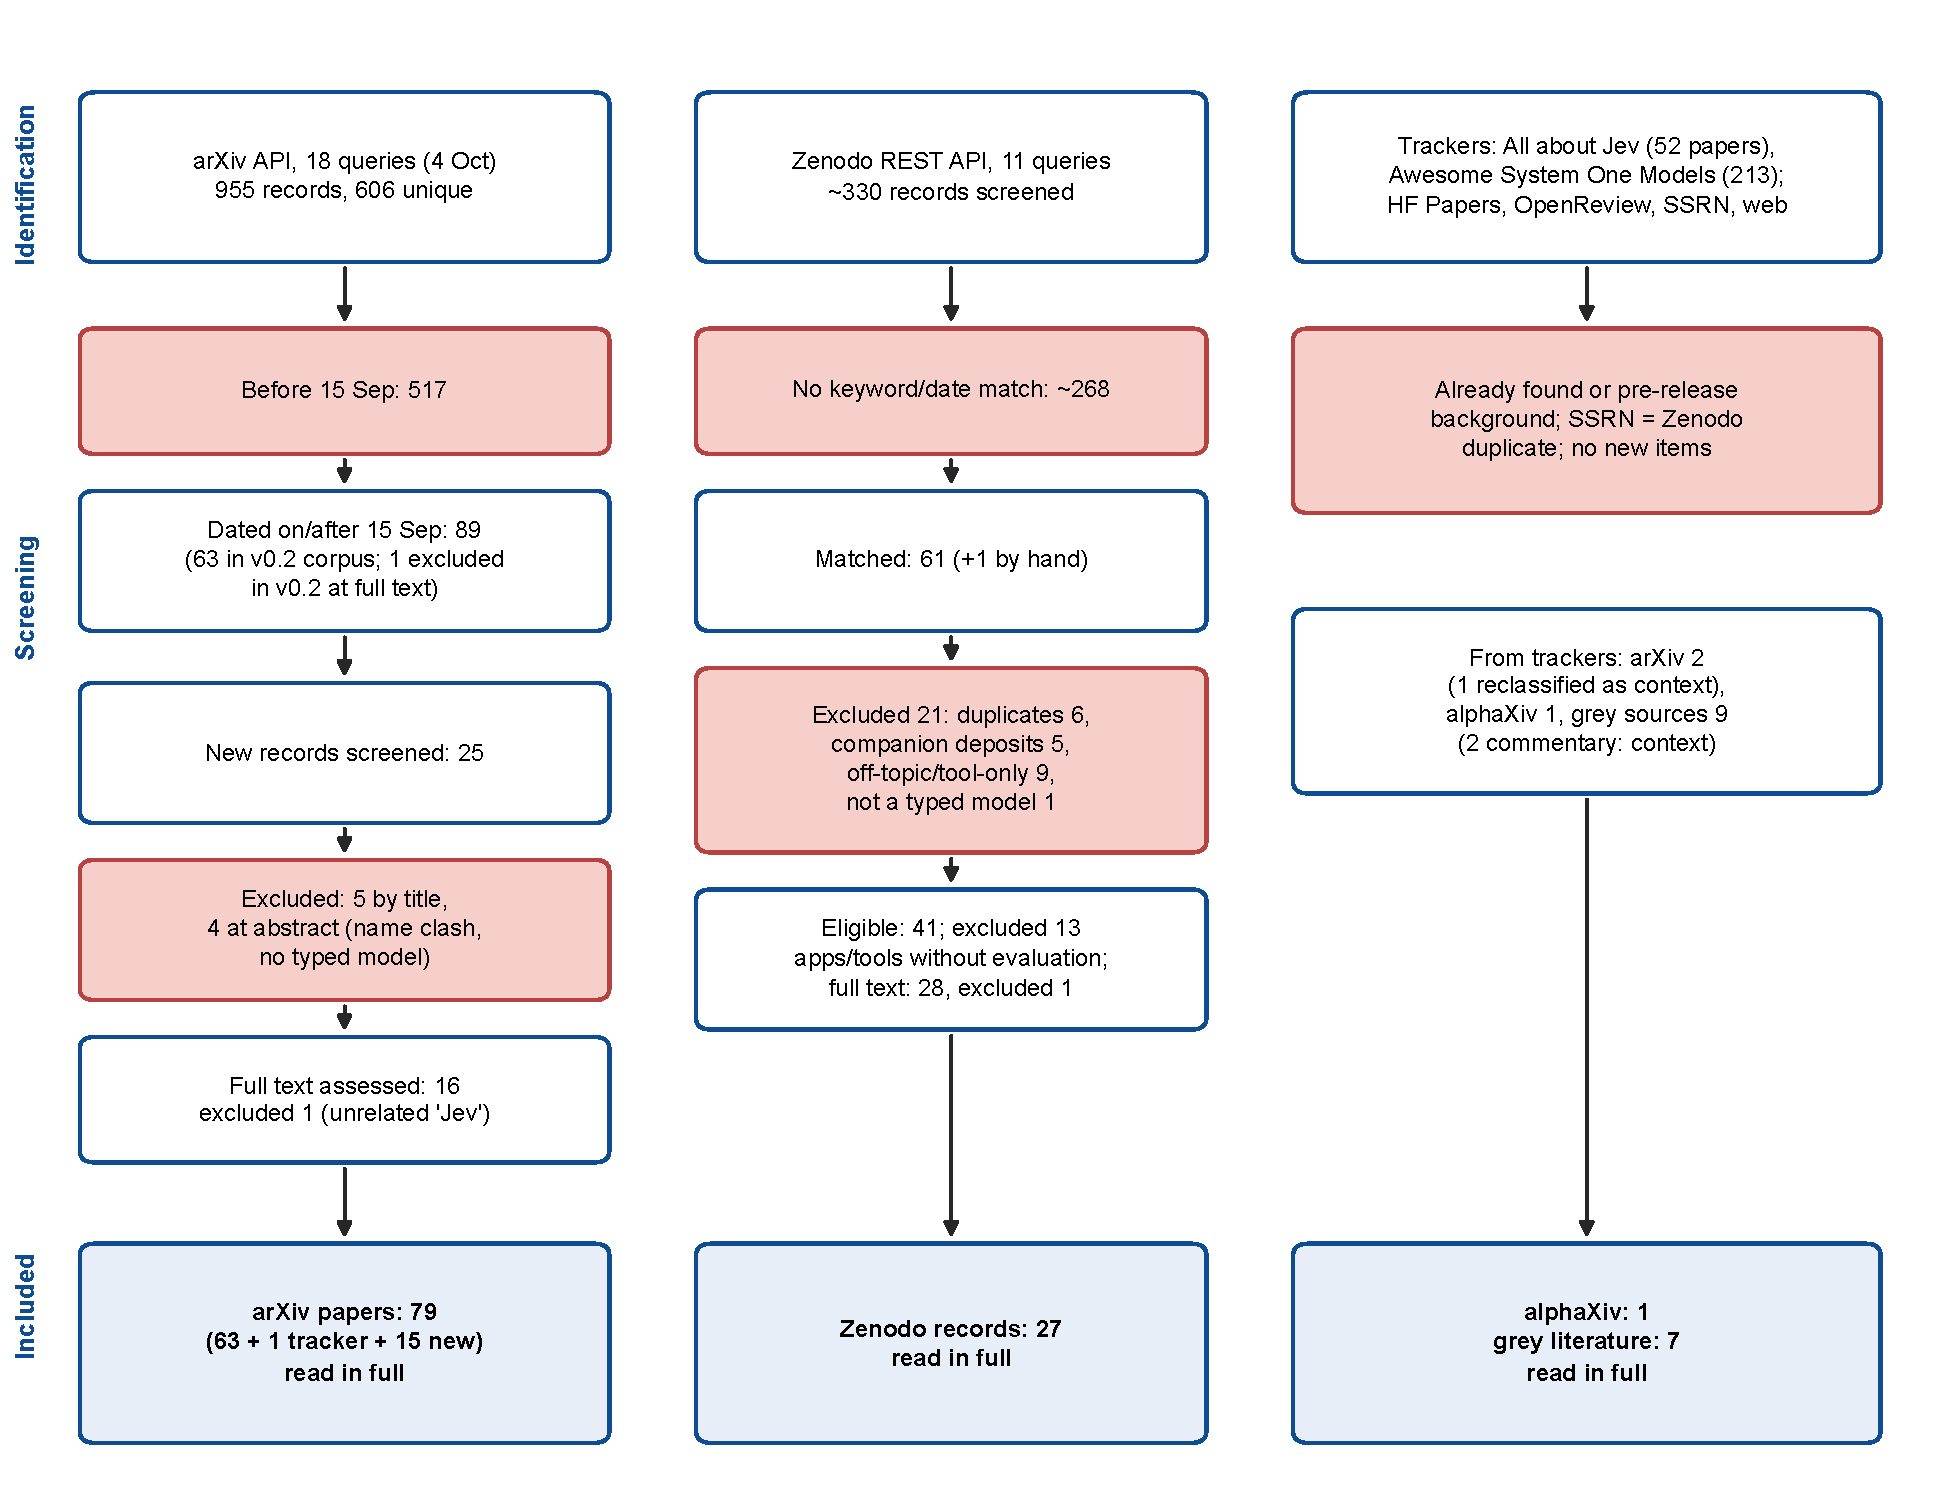
\includegraphics[width=0.85\linewidth]{figures/fig_prisma.pdf}
\caption{按来源划分的识别、筛选与纳入（PRISMA 2020 流程）。由于 API 返回的结果集相互重叠，Zenodo 在第一步的计数为近似值。}
\label{fig:prisma}
\end{figure}

\paragraph{PRISMA 2020 核查清单。}
\Cref{tab:prisma} 将 PRISMA~2020 声明的条目~\cite{page2021prisma}与本文内容逐一对应；未执行的条目均如实注明。

\begingroup
\small
\renewcommand{\arraystretch}{1.15}
\begin{longtable}{@{}p{0.30\linewidth}p{0.64\linewidth}@{}}
\caption{PRISMA 2020 条目及其报告位置。}\label{tab:prisma}\\
\toprule
条目 & 报告位置或状态 \\
\midrule
\endfirsthead
\toprule
条目 & 报告位置或状态 \\
\midrule
\endhead
\bottomrule
\endfoot
标题（1） & 按设计未遵循：本文是一项政策分析，其证据部分在\cref{sec:method}中被界定为结构化快速证据评估 \\
摘要（2） & 摘要陈述了问题、来源、方法、主要结果、确定性及其意义 \\
理由、目的（3--4） & \Cref{sec:intro}（研究问题） \\
纳入标准（5） & \Cref{sec:method}，纳入标准 \\
信息来源、检索（6--7） & \Cref{sec:method}；\cref{app:queries}；\nolinkurl{scripts/rerun_arxiv_search.py} \\
筛选过程（8） & \Cref{sec:method}（评审者与工具）：AI 智能体；无人工重复筛选 \\
数据收集、数据条目（9--10a/b） & \Cref{sec:method}，数据提取；\nolinkurl{data/evidence_coding.csv} \\
研究偏倚风险（11） & 设计评价（\cref{sec:appraisal}）；\nolinkurl{data/quality_appraisal.csv} \\
效应指标（12） & 不适用：按要求统计主要结果的方向；无合并效应 \\
综合：各项综合的纳入资格（13a） & 针对某项要求编码的研究（\cref{app:evidence}） \\
综合：数据准备（13b） & 编码与对照比较字段来自数据提取；未作转换 \\
综合：列表与展示（13c） & \Cref{fig:framework}、\cref{tab:keyfindings}与\cref{tab:evidence} \\
综合：方法（13d） & 按照 SWiM~\cite{campbell2020swim}对方向进行计票；未作 Meta 分析 \\
综合：异质性（13e） & 未作正式分析；任务和模型的异质性在\cref{sec:evidence}中描述 \\
综合：敏感性分析（13f） & 仅纳入设计较强的研究；排除 Zenodo 记录（\cref{sec:across}） \\
报告偏倚（14） & 未作正式评估；在\cref{sec:discussion}中讨论 \\
确定性评估（15） & GRADE 式规则（\cref{sec:appraisal}）；\cref{tab:keyfindings} \\
研究筛选（16a） & \Cref{fig:prisma} \\
看似符合条件但被排除的研究（16b） & \nolinkurl{data/excluded_records.csv}（例如无关的“Jev”论文、PDF 不符的记录以及不含类型化模型的测试框架论文） \\
研究特征（17） & \Cref{app:evidence,app:catalogue} \\
各研究的偏倚风险（18） & \Cref{tab:evidence}；\nolinkurl{data/quality_appraisal.csv} \\
单项研究结果（19） & \Cref{sec:evidence}；理由见 \nolinkurl{data/evidence_coding.csv} \\
综合结果（20a--d） & \Cref{sec:evidence,sec:across}；\cref{fig:framework}；未作异质性分析与正式检验 \\
报告偏倚（21） & 未作正式评估（\cref{sec:discussion}） \\
证据确定性（22） & \Cref{tab:keyfindings} \\
讨论（23a--d） & \Cref{sec:discussion}（解释、证据与过程的局限、意义） \\
注册与方案（24a--c） & 未注册；未发布方案；相对于早期发布的变更见\cref{sec:method} \\
资助（25） & 无资助 \\
利益冲突（26） & 立场声明与利益冲突声明 \\
数据、代码和材料的可获得性（27） & 数据与代码可获得性声明 \\
\end{longtable}
\endgroup

\bibliographystyle{unsrtnat}
\bibliography{../pol2,../corpus,../corpus_update,../grey,../background}
\end{document}
